%%%%%%%%%%%%%%%%%%%%%%%%%%%%%%%%%%%%%%%%%%%%%%%%%%%%%%%%%%%%%%%%%%%%%%%%%%%
% PFC/Tesis Latex Template
%%%%%%%%%%%%%%%%%%%%%%%%%%%%%%%%%%%%%%%%%%%%%%%%%%%%%%%%%%%%%%%%%%%%%%%%%%%
%%%%%%%%%%%%%%%%%%%%%%%%%%%%%%%%%%%%%%%%%%%%%%%%%%%%%%%%%%%%%%%%%%%%%%%%%%%
%
% Generic template for TFC/TFM/TFG/Tesis
%
% $Id: preamble.tex,v 1.9 2013/11/04 23:46:21 macias Exp $
%
% By:
%  + Javier Mac�as-Guarasa. 
%    Departamento de Electr�nica
%    Universidad de Alcal�
%  + Roberto Barra-Chicote. 
%    Departamento de Ingenier�a Electr�nica
%    Universidad Polit�cnica de Madrid   
% 
% Based on original sources by Roberto Barra, Manuel Oca�a, Jes�s Nuevo,
% Pedro Revenga, Fernando Herr�nz and Noelia Hern�ndez. Thanks a lot to
% all of them, and to the many anonymous contributors found (thanks to
% google) that provided help in setting all this up.
%
% If you think you can add pieces of relevant/useful examples,
% improvements, please contact us at (macias@depeca.uah.es)
%
% (copyleft)2013
%
%%%%%%%%%%%%%%%%%%%%%%%%%%%%%%%%%%%%%%%%%%%%%%%%%%%%%%%%%%%%%%%%%%%%%%%%%%%

\documentclass[svgnames,spanish,openright]{book}
%\documentclass[english,openright]{book}
%\documentclass[11pt,english,twoside,openright]{book}

%\usepackage[a4,cam,center]{crop}
%\crop[font=\upshape\mdseries\small\textsf]

\usepackage[latin1]{inputenc} % Para poder escribir con acentos y �.
\usepackage[T1]{fontenc}      % Para que haga bien la ``hyphenation''. No
                              % usar si no es necesario, porque ralentiza muchisimo la compilaci�n.
\usepackage{ae}               % Para que todas las fuentes sean Type1, y ninguna Type3.

\usepackage[spanish, english]{babel}

% Use this if you want to include pdf files in the final document
\usepackage[final]{pdfpages}

% Use this if you want to delete headers and footers in empty pages
\usepackage{emptypage}

%\usepackage[nottoc]{tocbibind}
\usepackage{tocbibind}

\usepackage{listings}
\usepackage{longtable}
\usepackage{afterpage}

\usepackage{xspace}
\usepackage{verbatim}
\usepackage{moreverb}
\usepackage{multicol}
\usepackage{amsmath}
\usepackage{eurosym}
\usepackage{subfigure}
\usepackage{multirow}
\usepackage{fancyhdr}
\usepackage{makeidx}
\usepackage{rotating}
\usepackage{supertabular}
\usepackage{hhline}
\usepackage{array}
\usepackage[noadjust]{cite}      % Written by Donald Arseneau
                        % V1.6 and later of IEEEtran pre-defines the format
                        % of the cite.sty package \cite{} output to follow
                        % that of IEEE. Loading the cite package will
                        % result in citation numbers being automatically
                        % sorted and properly "ranged". i.e.,
                        % [1], [9], [2], [7], [5], [6]
                        % (without using cite.sty)
                        % will become:
                        % [1], [2], [5]--[7], [9] (using cite.sty)
                        % cite.sty's \cite will automatically add leading
                        % space, if needed. Use cite.sty's noadjust option
                        % (cite.sty V3.8 and later) if you want to turn this
                        % off. cite.sty is already installed on most LaTeX
                        % systems. The latest version can be obtained at:
                        % http://www.ctan.org/tex-archive/macros/latex/contrib/supported/cite/


\usepackage[RGB,rgb]{xcolor}

% To draw rectagles in tfm cover
\usepackage{tikz}


%\usepackage[authoryear]{natbib}
% \makeatletter
% \let\NAT@parse\undefined
% \makeatother
% \usepackage{natbib}

\usepackage{geometry}
\geometry{verbose,a4paper,tmargin=2.5cm,bmargin=2.5cm,lmargin=2.5cm,rmargin=2.5cm}
%\geometry{paperwidth=210mm,paperheight=297mm}

\usepackage[
ps2pdf,                %%% hyper-references for ps2pdf
bookmarks=true,%                   %%% generate bookmarks ...
bookmarksnumbered=true,            %%% ... with numbers
hypertexnames=false,               %%% needed for correct links to
                                %%% figures!!!
%hypertexnames=true,               %%% needed for correct links on pagebackrefs!!!
breaklinks=true,                   %%% breaks lines, but links are very small
%pagebackref=true,
%linktocpage=true,                 %%% enlace en el numero de p�gina.
linktoc=all,
colorlinks=true,
linkcolor=azul,    
citecolor=verde,
urlcolor=azul,                     %%% texto  con color
linkbordercolor={0 0 1},           %%% blue frames around links
pdfborder={0 0 112.0}              %%% border-width of frames 
]{hyperref}                        %%% will be multiplied with 0.009 by ps2pdf


% Para numerar las \subsubsection
\setcounter{secnumdepth}{5}
%para hacer que las \subsubsection aparezcan en el indice
\setcounter{tocdepth}{5}
%\setcounter{lofdepth}{2}
\setcounter{table}{1}
\setcounter{figure}{1}
\setcounter{secnumdepth}{4}


\setlength{\parskip}{1ex plus 0.5ex minus 0.2ex}


\usepackage{multirow}

\usepackage{setspace}
% \renewcommand{\baselinestretch}{10}
\newcommand{\mycaptiontable}[1]{
\begin{spacing}{0.6}
  %\vspace{0.5cm}
  \begin{quote}
    %\begin{center}
            {{Table} \thechapter.\arabic{table}: #1}
    %\end{center}
  \end{quote}
  %\vspace{1cm}
  \end{spacing}
  \stepcounter{table}
}

\newcommand{\mycaptionfigure}[1]{
  %\vspace{0.5cm}
  \begin{spacing}{0.6}
  \begin{quote}
    %\begin{center}
            {{Figure} \thechapter.\arabic{figure}: #1}
    %\end{center}
  \end{quote}
  %\vspace{1cm}
  \end{spacing}
  \stepcounter{figure}
}

% \newlength{\myVSpace}% the height of the box
% \setlength{\myVSpace}{0ex}% the default, 
% \newcommand\xstrut{\raisebox{-.5\myVSpace}% symmetric behaviour, 
%   {\rule{0pt}{\myVSpace}}%
% }

\usepackage{amsmath}

\usepackage{courier}

%***************************************************************************
%***************************************************************************
%***************************************************************************
\usepackage{multirow}
\usepackage{rotating}
\usepackage{setspace, amssymb, amsmath, epsfig, multirow, colortbl, tabularx}%
% For acronym package:
% If footnote is specified, text will be included in a footnote
% If printonlyused is specified, only used acronyms will be included
% I use the acronym sty under the sty directory as I needed the newest version
%\usepackage[footnote,printonlyused,withpage]{acronym} 
%\usepackage[printonlyused]{sty/acronym}

% Mejor que el acronym es glossaries
\usepackage[acronym,shortcuts,nomain]{glossaries}

% ifthen to allow using language dependent settings
\usepackage{ifthen}

\newcommand{\clearemptydoublepage}{\newpage{\pagestyle{empty}\cleardoublepage}}


\pagestyle{fancy}

% Pantone 160
%\definecolor{headingPortadaTFM}{RGB}{158,84,10}
% Pantone 160C (this is supposed to be the correct one, but it looks horrible in screen)
%\definecolor{headingPortadaTFM}{RGB}{161,86,28}
% Gold in RGB
%\definecolor{textoHeadingPortadaTFM}{RGB}{215,215,0}
% Captured colors in screen (this looks pst on screen)
\definecolor{headingPortadaTFM}{RGB}{152,118,52}
\definecolor{textoHeadingPortadaTFM}{RGB}{208,205,102}

\definecolor{azul}{rgb}{0,0,1}
\definecolor{verde}{rgb}{0,0.5,0}
\definecolor{rojo}{rgb}{1,0,0}
\definecolor{cyan}{rgb}{0,0.75,0.75}
\definecolor{magenta}{rgb}{0.75,0,0.75}
\definecolor{amarillo}{rgb}{0.75,0.75,0}
\definecolor{gris}{rgb}{0.25,0.25,0.25}
\definecolor{r}{rgb}{0,0,1}
\definecolor{g}{rgb}{0,1,0}
\definecolor{b}{rgb}{1,0,0}
\definecolor{c}{rgb}{0,1,1}
\definecolor{m}{rgb}{1,0,1}
\definecolor{y}{rgb}{1,1,0}
\definecolor{w}{rgb}{1,1,1}
\definecolor{k}{rgb}{0,0,0}
\definecolor{azulE}{rgb}{0,0.3984,0.5977}
\definecolor{amarilloE}{rgb}{0.9961,0.7969,0}
\definecolor{blanco}{rgb}{1,1,1}
\definecolor{burdeos}{rgb}{1,0,0.95}


\providecommand\phantomsection{}
\onehalfspacing
\sloppy  %better line breaks

\renewcommand{\chaptermark}[1]{\markboth{\chaptername\ \thechapter.\ #1}{}}
\renewcommand{\sectionmark}[1]{\markright{\thesection\ #1}{}}



\fancyhf{}

\fancyhead[LE,RO]{\bfseries\thepage}
\fancyhead[LO]{\bfseries\rightmark}
\fancyhead[RE]{\bfseries\leftmark}

\renewcommand{\headrulewidth}{0.5pt}
\renewcommand{\footrulewidth}{0pt}
\addtolength{\headheight}{3.5pt}
\fancypagestyle{plain}{\fancyhead{}  
  \renewcommand{\headrulewidth}{0pt}}

%\makeglossaries

\fancypagestyle{myplain}
{
  \fancyhf{}
  \renewcommand\headrulewidth{0pt}
  \renewcommand\footrulewidth{0pt}
  \fancyfoot[C]{\thepage}
}

% To set background image in TFMs front and back pages
\usepackage[pages=some]{sty/background}

\backgroundsetup{ scale=1, angle=0, opacity=.1, color=pink,
  contents={
\includegraphics[width=.7\paperwidth]{logos/logoEPS-UAH.jpg}}, vshift=-50pt,  hshift=0pt }

\makeatletter
\newcommand*{\cleartoleftpage}{%
  \clearpage
    \if@twoside
    \ifodd\c@page
      \hbox{}\newpage
      \if@twocolumn
        \hbox{}\newpage
      \fi
    \fi
  \fi
}
\makeatother
    % All definitions, packages, etc.

%%%%%%%%%%%%%%%%%%%%%%%%%%%%%%%%%%%%%%%%%%%%%%%%%%%%%%%%%%%%%%%%%%%%%%%%%%%
%
% Generic template for TFC/TFM/TFG/Tesis
%
% $Id:$
%
% By:
%  + Javier Mac�as-Guarasa. 
%    Departamento de Electr�nica
%    Universidad de Alcal�
%  + Roberto Barra-Chicote. 
%    Departamento de Ingenier�a Electr�nica
%    Universidad Polit�cnica de Madrid   
% 
% Based on original sources by Roberto Barra, Manuel Oca�a, Jes�s Nuevo,
% Pedro Revenga, Fernando Herr�nz and Noelia Hern�ndez. Thanks a lot to
% all of them, and to the many anonymous contributors found (thanks to
% google) that provided help in setting all this up.
%
% If you think you can add pieces of relevant/useful examples,
% improvements, please contact us at (macias@depeca.uah.es)
%
% (copyleft)2013
%
%%%%%%%%%%%%%%%%%%%%%%%%%%%%%%%%%%%%%%%%%%%%%%%%%%%%%%%%%%%%%%%%%%%%%%%%%%%

%%%%%%%%%%%%%%%%%%%%%%%%%%%%%%%%%%%%%%%%%%%%%%%%%%%%%%%%%%%%%%%%%%%%%%%%%%% 
%
% Contents of this file:
% + Definition of your own commands (samples provided)
% + Definition of variables controlling compilation flavours
%
% You must edit it to suit to your specific case
%
% Specially important are the definition of your variables (title of the
% book, your degree, author name, email, advisors, keywords (in Spanish
% and English), year, ... They will be used in generating the adequate
% front and cover pages, automagically.
%
%%%%%%%%%%%%%%%%%%%%%%%%%%%%%%%%%%%%%%%%%%%%%%%%%%%%%%%%%%%%%%%%%%%%%%%%%%% 


%%%%%%%%%%%%%%%%%%%%%%%%%%%%%%%%%%%%%%%%%%%%%%%%%%%%%%%%%%%%%%%%%%%%%%%%%%% 
% BEGIN My own commands section 
% Define your own commands here

% This one is to define a specific format for english text in a Spanish
% document
\DeclareRobustCommand{\texten}[1]{\textit{#1}}

% Various examples
\newcommand{\circulo}{\large $\circ$}
\newcommand{\asterisco}{$\ast$}
\newcommand{\cuadrado}{\tiny $\square$}
\newcommand{\triangulo}{\scriptsize $\vartriangle$}
\newcommand{\triangv}{\scriptsize $\triangledown$}
\newcommand{\diamante}{\large $\diamond$}

\newcommand{\new}[1]{\textcolor{magenta}{#1 }}
\newcommand{\argmax}[1]{\underset{#1}{\operatorname{argmax}}}

% END My own commands section 
%%%%%%%%%%%%%%%%%%%%%%%%%%%%%%%%%%%%%%%%%%%%%%%%%%%%%%%%%%%%%%%%%%%%%%%%%%% 

%%%%%%%%%%%%%%%%%%%%%%%%%%%%%%%%%%%%%%%%%%%%%%%%%%%%%%%%%%%%%%%%%%%%%%%%%%% 
% BEGIN Set my own variables (control compilation for different flavours)

% Control language specific modifications
% This can be english or spanish
\newcommand{\mybooklanguage}{spanish}

% Control compilation flavour (for PFCs, TFMs, TFGs, Thesis, etc...)
% Degree (titulaci�n), can be:
% IT    - Ingenier�a de Telecomunicaci�n
% IE    - Ingenier�a Electr�nica
% ITTSE - Ingenier�a T�cnica de Telecomunicaci�n, Sistemas Electr�nicos
% ITTST - Ingenier�a T�cnica de Telecomunicaci�n, Sistemas de Telecomunicaci�n
% ITI   - Ingenier�a T�cnica Industrial, Electr�nica Industrial 
% GIEC  - Grado en Ingenier�a Electr�nica de Comunicaciones
% GIEAI - Grado en Ingenier�a en Electr�nica y Autom�tica Industrial
% GIST  - Grado en Ingenier�a en Sistemas de Telecomunicaci�n
% GITT  - Grado en Ingenier�a en Tecnolog�as de la Telecomunicaci�n
% GIT   - Grado en Ingenier�a Telem�tica
% GIC   - Grado en Ingenier�a de Computadores
% GII   - Grado en Ingenier�a Inform�tica
% GSI   - Grado en Sistemas de Informaci�n
% MUSEA - M�ster Universitario en Sistemas Electr�nicos Avanzados. Sistemas Inteligentes
% PHD   - Doctorado
\newcommand{\mydegree}{GIEC}

% General document information
\newcommand{\mybooktitle}{Title of the pfc/tfm/tfg/tesis}
\newcommand{\mybookauthor}{Full name of author}
\newcommand{\mybookemail}{autor@depeca.uah.es}
\newcommand{\mybookadvisors}{Full name of advisors}
\newcommand{\mybookyear}{Year of the examination}
\newcommand{\mybookkeywords}{First, second, third, fourth and fifth (up to a maximum of five)}
\newcommand{\mybookpalabrasclave}{Primera, segunda, tercera, cuarta y quinta (m�ximo de cinco)}

% END Set my own variables (control compilation for different flavours)
%%%%%%%%%%%%%%%%%%%%%%%%%%%%%%%%%%%%%%%%%%%%%%%%%%%%%%%%%%%%%%%%%%%%%%%%%%% 

    % EDIT IT! to set your specific settings!

%%%%%%%%%%%%%%%%%%%%%%%%%%%%%%%%%%%%%%%%%%%%%%%%%%%%%%%%%%%%%%%%%%%%%%%%%%%
%
% Generic template for TFC/TFM/TFG/Tesis
%
% $Id: glossaries.tex,v 1.4 2013/11/25 00:33:31 macias Exp $
%
% By:
%  + Javier Mac�as-Guarasa. 
%    Departamento de Electr�nica
%    Universidad de Alcal�
%  + Roberto Barra-Chicote. 
%    Departamento de Ingenier�a Electr�nica
%    Universidad Polit�cnica de Madrid   
% 
% Based on original sources by Roberto Barra, Manuel Oca�a, Jes�s Nuevo,
% Pedro Revenga, Fernando Herr�nz and Noelia Hern�ndez. Thanks a lot to
% all of them, and to the many anonymous contributors found (thanks to
% google) that provided help in setting all this up.
%
% See also the additionalContributors.txt file to check the name of
% additional contributors to this work.
%
% If you think you can add pieces of relevant/useful examples,
% improvements, please contact us at (macias@depeca.uah.es)
%
% Copyleft 2013
%
%%%%%%%%%%%%%%%%%%%%%%%%%%%%%%%%%%%%%%%%%%%%%%%%%%%%%%%%%%%%%%%%%%%%%%%%%%%


% Define a new glossary type for symbols used in equations (example)
\newglossary[slg]{symbols}{sym}{sbl}{List of Symbols}

\makeglossaries               % DO NOT TOUCH THIS!


%%% Local Variables:
%%% TeX-master: "../book"
%%% End:


  % EDIT IT to include your glossaries!

%%%%%%%%%%%%%%%%%%%%%%%%%%%%%%%%%%%%%%%%%%%%%%%%%%%%%%%%%%%%%%%%%%%%%%%%%%%
%
% Generic template for TFC/TFM/TFG/Tesis
%
% $Id: postamble.tex,v 1.16 2017/04/06 13:56:12 macias Exp $
%
% By:
%  + Javier Mac�as-Guarasa. 
%    Departamento de Electr�nica
%    Universidad de Alcal�
%  + Roberto Barra-Chicote. 
%    Departamento de Ingenier�a Electr�nica
%    Universidad Polit�cnica de Madrid   
% 
% Based on original sources by Roberto Barra, Manuel Oca�a, Jes�s Nuevo,
% Pedro Revenga, Fernando Herr�nz and Noelia Hern�ndez. Thanks a lot to
% all of them, and to the many anonymous contributors found (thanks to
% google) that provided help in setting all this up.
%
% See also the additionalContributors.txt file to check the name of
% additional contributors to this work.
%
% If you think you can add pieces of relevant/useful examples,
% improvements, please contact us at (macias@depeca.uah.es)
%
% You can freely use this template and please contribute with
% comments or suggestions!!!
%
%%%%%%%%%%%%%%%%%%%%%%%%%%%%%%%%%%%%%%%%%%%%%%%%%%%%%%%%%%%%%%%%%%%%%%%%%%%

%%%%%%%%%%%%%%%%%%%%%%%%%%%%%%%%%%%%%%%%%%%%%%%%%%%%%%%%%%%%%%%%%%%%%%%%%%%
%
% You should not need to edit this file. Yes, I know the name is not a
% valid word... :-)
%
% Here we define \mydegreefull, \mybookworktype and \mybookworktypefull 
% that will be used by other modules. The decision is based on the
% \mydegree variable set by the user.
%
% In case the \mydegree variable is now known, the module will generate 
% an error message in \mydegreefull and \mybookworktypefull, but will 
% generate a valid \mybookworktype, to be able to generate front and
% cover pages (TFG by default)
%
%%%%%%%%%%%%%%%%%%%%%%%%%%%%%%%%%%%%%%%%%%%%%%%%%%%%%%%%%%%%%%%%%%%%%%%%%%%

\ifthenelse{\equal{\mybooklanguage}{spanish}}
{
\usepackage[spanish]{babel}
\newcommand{\mybookFullAffiliation}{Grupo de investigaci�n \mybookresearchgroup \\ \mybookdepartment \\ \mybookuniversity} 
\newcommand{\mybooktitle}{\mybooktitlespanish}
} 
{
\usepackage[english]{babel}
\newcommand{\mybookFullAffiliation}{\mybookresearchgroup Research Group \\ \mybookdepartmentEnglish \\ \mybookuniversity} 
\newcommand{\mybooktitle}{\mybooktitleenglish}
}

\ifthenelse{\equal{\mybooklanguage}{spanish}}
{
\newcommand{\andOrY}{y} 
} 
{
\newcommand{\andOrY}{and} 
}

% Sex issues
\ifthenelse{\equal{\mybookAcademicTutorSex}{male}}     
{                                                       
\newcommand{\donOrDonaTutor}{D.}
\newcommand{\drOrDraTutor}{Dr.}
}
{
\newcommand{\donOrDonaTutor}{D�.}
\newcommand{\drOrDraTutor}{Dra.}
}

\ifthenelse{\equal{\mybookCoTutorSex}{male}}     
{                                                       
\newcommand{\donOrDonaCoTutor}{D.}
\newcommand{\drOrDraCoTutor}{Dr.}
}
{
\newcommand{\donOrDonaCoTutor}{D�.}
\newcommand{\drOrDraCoTutor}{Dra.}
}

\ifthenelse{\equal{\mybookauthorsex}{male}}     
{                                                       
\newcommand{\donOrDonaAutor}{D.}
}
{
\newcommand{\donOrDonaAutor}{D�.}
}

% Set name of advisors and define words depending on singular/plural
\ifthenelse{\equal{\mybookNameCoTutor}{}}
{
\newcommand{\mybookadvisors}{\mybookNameAcademicTutor{}}
\newcommand{\mybookadvisorsConDon}{\donOrDonaTutor{} \mybookNameAcademicTutor{}}
\newcommand{\mybookadvisorsConDr}{\drOrDraTutor{} \mybookNameAcademicTutor{}}
\ifthenelse{\equal{\mybookAcademicTutorSex}{male}}     
{                                                       
\newcommand{\directorOrdirectora}{director}
\newcommand{\mybookTutorOrTutores}{tutor}
}
{
\newcommand{\directorOrdirectora}{directora}
\newcommand{\mybookTutorOrTutores}{tutora}
}
\newcommand{\mybookDirectorOrDirectores}{\directorOrdirectora}
\newcommand{\mybookAdvisorOrAdvisors}{advisor}
\newcommand{\mybookDaOrDan}{da}
\newcommand{\mybookEmiteOrEmiten}{emite}
\newcommand{\mybookElOrLos}{El}
\newcommand{\mybookSuOrSus}{su}
\newcommand{\mybookDelOrDeLos}{del}
\newcommand{\mybookHagoOrHacemos}{hago}
}
{
\newcommand{\mybookadvisors}{\mybookNameAcademicTutor{} \andOrY{} \mybookNameCoTutor{}}
\newcommand{\mybookadvisorsConDon}{\donOrDonaTutor{} \mybookNameAcademicTutor{} \andOrY{} \donOrDonaCoTutor{} \mybookNameCoTutor{}}
\newcommand{\mybookadvisorsConDr}{\drOrDraTutor{} \mybookNameAcademicTutor{}\\\drOrDraCoTutor{} \mybookNameCoTutor{}}

\newcommand{\mybookDirectorOrDirectores}{directores}
\newcommand{\mybookAdvisorOrAdvisors}{advisors}
\newcommand{\mybookDaOrDan}{dan}
\newcommand{\mybookEmiteOrEmiten}{emiten}
\newcommand{\mybookTutorOrTutores}{tutores}
\newcommand{\mybookElOrLos}{Los}
\newcommand{\mybookSuOrSus}{Su}
\newcommand{\mybookDelOrDeLos}{de los}
\newcommand{\mybookHagoOrHacemos}{hacemos}
}

% Set Autor/Autora field
\ifthenelse{\equal{\mybookauthorsex}{male}}     
{                                                       
\newcommand{\mybookAutorOrAutora}{autor}                
\newcommand{\mybookElOrLa}{el}                
\newcommand{\mybookAlOrALa}{al}                
\newcommand{\mybookDelOrDeLa}{del}                
\newcommand{\mybookDonOrDona}{D}                
\newcommand{\mybookNotificadoOrNotificada}{notificado}                
\newcommand{\mybookAdscritoOrAdscrita}{adscrito}                
\newcommand{\mybookAlumnoOrAlumna}{alumno}                
}                                               
{
\newcommand{\mybookAutorOrAutora}{autora}                
\newcommand{\mybookElOrLa}{la}                
\newcommand{\mybookAlOrALa}{a la}                
\newcommand{\mybookDelOrDeLa}{de la}                
\newcommand{\mybookDonOrDona}{D�}                
\newcommand{\mybookNotificadoOrNotificada}{notificada}    
\newcommand{\mybookAdscritoOrAdscrita}{adscrita}                
\newcommand{\mybookAlumnoOrAlumna}{alumna}                            
}

% Set degree name and type of document, depending on the user defined degree
\ifthenelse{\equal{\mydegree}{IT}}
{
  \newcommand{\mydegreefull}{Ingenier�a de Telecomunicaci�n}
  \newcommand{\mybookworktype}{TFC}
  \ifthenelse{\equal{\mybooklanguage}{spanish}}
  {
    \newcommand{\mybookworktypefull}{Trabajo Fin de Carrera}
  }
  {
    % This could be translated. I'm leaving this in Spanish...
    % \newcommand{\mybookworktypefull}{Master's Thesis}
    \newcommand{\mybookworktypefull}{Trabajo Fin de Carrera}
  }
}
{
  \ifthenelse{\equal{\mydegree}{IE}}
  {
    \newcommand{\mydegreefull}{Ingenier�a Electr�nica}
    \newcommand{\mybookworktype}{TFC}
    \ifthenelse{\equal{\mybooklanguage}{spanish}}
    {
      \newcommand{\mybookworktypefull}{Trabajo Fin de Carrera}
    }
    {
      % This could be translated. I'm leaving this in Spanish...
      % \newcommand{\mybookworktypefull}{Master's Thesis}
      \newcommand{\mybookworktypefull}{Trabajo Fin de Carrera}
    }
  }
  {
    \ifthenelse{\equal{\mydegree}{ITTSE}}
    {
      \newcommand{\mydegreefull}{Ingenier�a T�cnica de Telecomunicaci�n, especialidad en Sistemas Electr�nicos}
      \newcommand{\mybookworktype}{TFC}
      \ifthenelse{\equal{\mybooklanguage}{spanish}}
      {
        \newcommand{\mybookworktypefull}{Trabajo Fin de Carrera}
      }
      {
        % This could be translated. I'm leaving this in Spanish...
        % \newcommand{\mybookworktypefull}{Bachelor's Thesis}
        \newcommand{\mybookworktypefull}{Trabajo Fin de Carrera}
      }
    }
    {
      \ifthenelse{\equal{\mydegree}{ITTST}}
      {
        \newcommand{\mydegreefull}{Ingenier�a T�cnica de Telecomunicaci�n, especialidad en Sistemas de Telecomunicaci�n}
      \newcommand{\mybookworktype}{TFC}
        \ifthenelse{\equal{\mybooklanguage}{spanish}}
        {
          \newcommand{\mybookworktypefull}{Trabajo Fin de Carrera}
        }
        {
          % This could be translated. I'm leaving this in Spanish...
          % \newcommand{\mybookworktypefull}{Bachelor's Thesis}
          \newcommand{\mybookworktypefull}{Trabajo Fin de Carrera}
        }
      }
      {
        \ifthenelse{\equal{\mydegree}{ITI}}
        {
          \newcommand{\mydegreefull}{Ingenier�a T�cnica Industrial, especialidad en Electr�nica Industrial}
          \newcommand{\mybookworktype}{TFC}
          \ifthenelse{\equal{\mybooklanguage}{spanish}}
          {
            \newcommand{\mybookworktypefull}{Trabajo Fin de Carrera}
          }
          {
            % This could be translated. I'm leaving this in Spanish...
            % \newcommand{\mybookworktypefull}{Bachelor's Thesis}
            \newcommand{\mybookworktypefull}{Trabajo Fin de Carrera}
          }
        }
        {
          \ifthenelse{\equal{\mydegree}{GIEC}}
          {
            \newcommand{\mydegreefull}{Grado en Ingenier�a Electr�nica de Comunicaciones}
            \newcommand{\mybookworktype}{TFG}
            \ifthenelse{\equal{\mybooklanguage}{spanish}}
            {
              \newcommand{\mybookworktypefull}{Trabajo Fin de Grado}
            }
            {
              % This could be translated. I'm leaving this in Spanish...
              % \newcommand{\mybookworktypefull}{Bachelor's Thesis}
              \newcommand{\mybookworktypefull}{Trabajo Fin de Grado}
            }
          }
          {
            \ifthenelse{\equal{\mydegree}{GIEAI}}
            {
              \newcommand{\mydegreefull}{Grado en Ingenier�a en Electr�nica y Autom�tica Industrial}
              \newcommand{\mybookworktype}{TFG}
              \ifthenelse{\equal{\mybooklanguage}{spanish}}
              {
                \newcommand{\mybookworktypefull}{Trabajo Fin de Grado}
              }
              {
                % This could be translated. I'm leaving this in Spanish...
                % \newcommand{\mybookworktypefull}{Bachelor's Thesis}
                \newcommand{\mybookworktypefull}{Trabajo Fin de Grado}
              }
            }
            {
              \ifthenelse{\equal{\mydegree}{GIST}}
              {
                \newcommand{\mydegreefull}{Grado en Ingenier�a en Sistemas de Telecomunicaci�n}
                \newcommand{\mybookworktype}{TFG}
                \ifthenelse{\equal{\mybooklanguage}{spanish}}
                {
                  \newcommand{\mybookworktypefull}{Trabajo Fin de Grado}
                }
                {
                  % This could be translated. I'm leaving this in Spanish...
                  % \newcommand{\mybookworktypefull}{Bachelor's Thesis}
                  \newcommand{\mybookworktypefull}{Trabajo Fin de Grado}
                }
              }
              {
                \ifthenelse{\equal{\mydegree}{GITT}}
                {
                  \newcommand{\mydegreefull}{Grado en Ingenier�a en Tecnolog�as de la Telecomunicaci�n}
                  \newcommand{\mybookworktype}{TFG}
                  \ifthenelse{\equal{\mybooklanguage}{spanish}}
                  {
                    \newcommand{\mybookworktypefull}{Trabajo Fin de Grado}
                  }
                  {
                    % This could be translated. I'm leaving this in Spanish...
                    % \newcommand{\mybookworktypefull}{Bachelor's Thesis}
                    \newcommand{\mybookworktypefull}{Trabajo Fin de Grado}
                  }
                }
                {
                  \ifthenelse{\equal{\mydegree}{GIT}}
                  {
                    \newcommand{\mydegreefull}{Grado en Ingenier�a Telem�tica}
                    \newcommand{\mybookworktype}{TFG}
                    \ifthenelse{\equal{\mybooklanguage}{spanish}}
                    {
                      \newcommand{\mybookworktypefull}{Trabajo Fin de Grado}
                    }
                    {
                      % This could be translated. I'm leaving this in Spanish...
                      % \newcommand{\mybookworktypefull}{Bachelor's Thesis}
                      \newcommand{\mybookworktypefull}{Trabajo Fin de Grado}
                    }
                  }
                  {
                    \ifthenelse{\equal{\mydegree}{GIC}}
                    {
                      \newcommand{\mydegreefull}{Grado en Ingenier�a de Computadores}
                      \newcommand{\mybookworktype}{TFG}
                      \ifthenelse{\equal{\mybooklanguage}{spanish}}
                      {
                        \newcommand{\mybookworktypefull}{Trabajo Fin de Grado}
                      }
                      {
                        % This could be translated. I'm leaving this in Spanish...
                        % \newcommand{\mybookworktypefull}{Bachelor's Thesis}
                        \newcommand{\mybookworktypefull}{Trabajo Fin de Grado}
                      }
                    }
                    {
                      \ifthenelse{\equal{\mydegree}{GII}}
                      {
                        \newcommand{\mydegreefull}{Grado en Ingenier�a Inform�tica}
                        \newcommand{\mybookworktype}{TFG}
                        \ifthenelse{\equal{\mybooklanguage}{spanish}}
                        {
                          \newcommand{\mybookworktypefull}{Trabajo Fin de Grado}
                        }
                        {
                          % This could be translated. I'm leaving this in Spanish...
                          % \newcommand{\mybookworktypefull}{Bachelor's Thesis}
                          \newcommand{\mybookworktypefull}{Trabajo Fin de Grado}
                        }
                      }
                      {
                        \ifthenelse{\equal{\mydegree}{GSI}}
                        {
                          \newcommand{\mydegreefull}{Grado en Sistemas de Informaci�n}
                          \newcommand{\mybookworktype}{TFG}
                          \ifthenelse{\equal{\mybooklanguage}{spanish}}
                          {
                            \newcommand{\mybookworktypefull}{Trabajo Fin de Grado}
                          }
                          {
                            % This could be translated. I'm leaving this in Spanish...
                            % \newcommand{\mybookworktypefull}{Bachelor's Thesis}
                            \newcommand{\mybookworktypefull}{Trabajo Fin de Grado}
                          }
                        }
                        {
                          \ifthenelse{\equal{\mydegree}{MUSEA}}
                          {
                            \newcommand{\mydegreefull}{M�ster Universitario en Sistemas Electr�nicos Avanzados. Sistemas Inteligentes}
                            \newcommand{\mydegreefullwrapped}{M�ster Universitario en Sistemas Electr�nicos Avanzados\\Sistemas Inteligentes}
                            \newcommand{\mydegreefullwrappedUpcase}{\MakeUppercase{M�ster Universitario en}\\\MakeUppercase{Ingenier�a de Telecomunicaci�n}}
                            \newcommand{\mybookworktype}{TFM}
                            \ifthenelse{\equal{\mybooklanguage}{spanish}}
                            {
                              \newcommand{\mybookworktypefull}{Trabajo Fin de M�ster}
                            }
                            {
                              % This could be translated. I'm leaving this in Spanish...
                              % \newcommand{\mybookworktypefull}{Master's Thesis}
                              \newcommand{\mybookworktypefull}{Trabajo Fin de M�ster}
                            }
                          }
                          {
                            \ifthenelse{\equal{\mydegree}{PHDUAH}}
                            {
                              \newcommand{\mydegreefull}{Estudios de Doctorado}
                              \newcommand{\mybookworktype}{PHDUAH}
                              \ifthenelse{\equal{\mybooklanguage}{spanish}}
                              {
                                \newcommand{\mybookworktypefull}{Tesis Doctoral}
                              }
                              {
                                \newcommand{\mybookworktypefull}{Doctoral Thesis}
                              }
                            }
                            {
                              \ifthenelse{\equal{\mydegree}{PHDUPM}}
                              {
                                \newcommand{\mydegreefull}{Doctor Ingeniero de Telecomunicaci�n}
                                \newcommand{\mybookworktype}{PHDUPM}
                                \ifthenelse{\equal{\mybooklanguage}{spanish}}
                                {
                                  \newcommand{\mybookworktypefull}{Tesis Doctoral}
                                }
                                {
                                  \newcommand{\mybookworktypefull}{Doctoral Thesis}
                                }
                              }
                              {
                                \ifthenelse{\equal{\mydegree}{GEINTRARR}}
                                {
                                  \newcommand{\mydegreefull}{GEINTRA Research Report}
                                  \newcommand{\mybookworktype}{GEINTRARR}
                                  \ifthenelse{\equal{\mybooklanguage}{spanish}}
                                  {
                                    \newcommand{\mybookworktypefull}{Informe t�cnico del Grupo de investigaci�n \mybookresearchgroup{}}
                                  }
                                  {
                                    \newcommand{\mybookworktypefull}{\mybookresearchgroup{} Research Report}
                                  }
                                }
                                {
                                  \ifthenelse{\equal{\mydegree}{MUIT}}
                                  {
                                    \newcommand{\mydegreefull}{M�ster Universitario en Ingenier�a de Telecomunicaci�n}
                                    \newcommand{\mydegreefullwrapped}{M�ster Universitario en Ingenier�a de Telecomunicaci�n}
                                    \newcommand{\mydegreefullwrappedUpcase}{\MakeUppercase{M�ster Universitario en}\\\MakeUppercase{Ingenier�a de Telecomunicaci�n}}
                                    \newcommand{\mybookworktype}{TFM}
                                    \ifthenelse{\equal{\mybooklanguage}{spanish}}
                                    {
                                    \newcommand{\mybookworktypefull}{Trabajo Fin de M�ster}
                                    }
                                    {
                                    % This could be translated. I'm leaving this in Spanish...
                                    % \newcommand{\mybookworktypefull}{Master's Thesis}
                                    \newcommand{\mybookworktypefull}{Trabajo Fin de M�ster}
                                    }
                                 }
                                 {
                                   \ifthenelse{\equal{\mydegree}{MUII}}
                                   {
                                     \newcommand{\mydegreefull}{M�ster Universitario en Ingenier�a Industrial}
                                     \newcommand{\mydegreefullwrapped}{M�ster Universitario en Ingenier�a Industrial}
                                     \newcommand{\mydegreefullwrappedUpcase}{\MakeUppercase{M�ster Universitario en}\\\MakeUppercase{Ingenier�a Industrial}}
                                     \newcommand{\mybookworktype}{TFM}
                                     \ifthenelse{\equal{\mybooklanguage}{spanish}}
                                     {
                                       \newcommand{\mybookworktypefull}{Trabajo Fin de M�ster}
                                     }
                                     {        
                                     % This could be translated. I'm leaving this in Spanish...
                                     % \newcommand{\mybookworktypefull}{Master's Thesis}
                                     \newcommand{\mybookworktypefull}{Trabajo Fin de M�ster}
                                     }
                                   }
                                   {
                                   \newcommand{\mybookworktype}{TFG}
                                   \newcommand{\mydegreefull}{ERROR: Defined degree (\mydegree) unknown, check \texttt{config/myconfig.tex}} 
                                   \newcommand{\mybookworktypefull}{ERROR: Defined degree (\mydegree) unknown, check \texttt{config/myconfig.tex}}
                                   }
                                 }
                               
                                }                               
                              }                          
                            }                          
                          }                          
                        }
                      }
                    }
                  }
                }
              }
            }
          }
        }
      }
    }
  }
}




%%%%%%%%%%%%%%%%%%%%%%%%%%%%%%%%%%%%%%%%%%%%%%%%%%%%%%%%%%%%%%%%%%%%%%%%%%%
% BEGIN Definition of the pdf document information data

\newcommand{\contactauthor}{\mybookauthor~\textless\href{mailto:\mybookemail}{\mybookemail}\textgreater}

% Set keywords for pdf information
\ifthenelse{\equal{\mybooklanguage}{english}}
{
  \newcommand{\keywordsforpdf}{\mybookkeywords}
}
{
  \newcommand{\keywordsforpdf}{\mybookpalabrasclave}
}

\newcommand{\underscoreSpacingFour}{\_\_\_\_}
\newcommand{\spacingFour}{~~~~}

\hypersetup
{
  pdfauthor={\mybookauthor~\textless\href{mailto:\mybookemail}{\mybookemail}\textgreater},
  pdftitle={\mybooktitle},
  pdfsubject={\mydegreefull, \mybookworktypefull},
% Uncomment the English or Spanish version if you wish to hard-code them
%  pdfkeywords={\mybookkeywords, \mybookworktypefull, \mydegreefull},
%  pdfkeywords={\mybookpalabrasclave, \mybookworktypefull, \mydegreefull},
  pdfkeywords={\keywordsforpdf},
  pdfcreator={\LaTeX with hyperref package},
  pdfproducer={rubber},
  pdffitwindow={true},
% This can be set in myconfig.tex
  urlcolor=\myurlcolor,
  linkcolor=\mylinkcolor,
  citecolor=\mycitecolor
}

% END Definition of the pdf document information data
%%%%%%%%%%%%%%%%%%%%%%%%%%%%%%%%%%%%%%%%%%%%%%%%%%%%%%%%%%%%%%%%%%%%%%%%%%%

%%% Local Variables:
%%% TeX-master: "../book"
%%% End:


   % DO NOT TOUCH THIS LINE

% ruta de las im�genes
\graphicspath{{./logos/}{./results/}{./diagrams/}}

%%%%%%%%%%%%%%%%%%%%%%%%%%%%%%%%%%%%%%%%%%%%%%%%%%%%%%%%%%%%%%%%%%%%%%%%%%%
% Let's start with the real stuff
%%%%%%%%%%%%%%%%%%%%%%%%%%%%%%%%%%%%%%%%%%%%%%%%%%%%%%%%%%%%%%%%%%%%%%%%%%%
\begin{document}

% Now start text and numbering for toc, list of tables/figures,...
\frontmatter

% Set Language dependent issues that must be set after \begin{document}
%%%%%%%%%%%%%%%%%%%%%%%%%%%%%%%%%%%%%%%%%%%%%%%%%%%%%%%%%%%%%%%%%%%%%%%%%%%
%
% Generic template for TFC/TFM/TFG/Tesis
%
% $Id: setlanguagedependentissues.tex,v 1.9 2015/02/24 23:21:55 macias Exp $
%
% By:
%  + Javier Mac�as-Guarasa. 
%    Departamento de Electr�nica
%    Universidad de Alcal�
%  + Roberto Barra-Chicote. 
%    Departamento de Ingenier�a Electr�nica
%    Universidad Polit�cnica de Madrid   
% 
% Based on original sources by Roberto Barra, Manuel Oca�a, Jes�s Nuevo,
% Pedro Revenga, Fernando Herr�nz and Noelia Hern�ndez. Thanks a lot to
% all of them, and to the many anonymous contributors found (thanks to
% google) that provided help in setting all this up.
%
% See also the additionalContributors.txt file to check the name of
% additional contributors to this work.
%
% If you think you can add pieces of relevant/useful examples,
% improvements, please contact us at (macias@depeca.uah.es)
%
% You can freely use this template and please contribute with
% comments or suggestions!!!
%
%%%%%%%%%%%%%%%%%%%%%%%%%%%%%%%%%%%%%%%%%%%%%%%%%%%%%%%%%%%%%%%%%%%%%%%%%%%

%%%%%%%%%%%%%%%%%%%%%%%%%%%%%%%%%%%%%%%%%%%%%%%%%%%%%%%%%%%%%%%%%%%%%%%%%%%
%
% You should not need to modify this file, unless you want to add
% language specific definitions.
%
%%%%%%%%%%%%%%%%%%%%%%%%%%%%%%%%%%%%%%%%%%%%%%%%%%%%%%%%%%%%%%%%%%%%%%%%%%%

\ifthenelse{\equal{\mybooklanguage}{english}}
{
  \selectlanguage{english}

  \newcommand{\xUseSpanish}{~}    
  \newcommand{\xUseEnglish}{X}  

  \floatname{codefloat}{Listing}
  \renewcommand{\lstlistingname}{Listing}

  %% \DeclareFloatingEnvironment[
  %%       fileext=lox,
  %%       listname={Source code listing},
  %%       name=Code,
  %%       placement=p,
  %%       within=section,
  %%       chapterlistsgaps=off,
  %%       ]{sourcecode}
}
{
  \selectlanguage{spanish}

  \newcommand{\xUseSpanish}{X}    
  \newcommand{\xUseEnglish}{~}  
  \renewcommand{\tablename}{Tabla}
  \renewcommand{\listtablename}{�ndice de tablas}

  \floatname{codefloat}{Listado}
  \renewcommand{\lstlistingname}{Listado}


  %% \DeclareFloatingEnvironment[
  %%       fileext=lox,
  %%       listname={Lista de c�digo fuente},
  %%       name=C�digo,
  %%       placement=p,
  %%       within=section,
  %%       chapterlistsgaps=off,
  %%       ]{sourcecode}
}

%%% Local Variables:
%%% TeX-master: "../book"
%%% End:


 % DO NOT TOUCH THIS LINE

% This will include front page (if needed), and cover pages
%%%%%%%%%%%%%%%%%%%%%%%%%%%%%%%%%%%%%%%%%%%%%%%%%%%%%%%%%%%%%%%%%%%%%%%%%%%
%
% Generic template for TFC/TFM/TFG/Tesis
%
% $Id: cover.tex,v 1.2 2013/11/04 23:46:21 macias Exp $
%
% By:
%  + Javier Mac�as-Guarasa. 
%    Departamento de Electr�nica
%    Universidad de Alcal�
%  + Roberto Barra-Chicote. 
%    Departamento de Ingenier�a Electr�nica
%    Universidad Polit�cnica de Madrid   
% 
% Based on original sources by Roberto Barra, Manuel Oca�a, Jes�s Nuevo,
% Pedro Revenga, Fernando Herr�nz and Noelia Hern�ndez. Thanks a lot to
% all of them, and to the many anonymous contributors found (thanks to
% google) that provided help in setting all this up.
%
% If you think you can add pieces of relevant/useful examples,
% improvements, please contact us at (macias@depeca.uah.es)
%
% Copyleft 2013
%
%%%%%%%%%%%%%%%%%%%%%%%%%%%%%%%%%%%%%%%%%%%%%%%%%%%%%%%%%%%%%%%%%%%%%%%%%%%

%%%%%%%%%%%%%%%%%%%%%%%%%%%%%%%%%%%%%%%%%%%%%%%%%%%%%%%%%%%%%%%%%%%%%%%%%%% 
% Defines the cover to be used depending on the type of work (that is
% turn depends on the \mydegree variable
%%%%%%%%%%%%%%%%%%%%%%%%%%%%%%%%%%%%%%%%%%%%%%%%%%%%%%%%%%%%%%%%%%%%%%%%%%%

\ifthenelse{\equal{\mybookworktype}{TFG}}
{
  %%%%%%%%%%%%%%%%%%%%%%%%%%%%%%%%%%%%%%%%%%%%%%%%%%%%%%%%%%%%%%%%%%%%%%%%%%%
%
% Generic template for TFC/TFM/TFG/Tesis
%
% $Id: portada-tfg-uah.tex,v 1.13 2018/12/12 13:48:22 macias Exp $
%
% By:
%  + Javier Mac�as-Guarasa. 
%    Departamento de Electr�nica
%    Universidad de Alcal�
%  + Roberto Barra-Chicote. 
%    Departamento de Ingenier�a Electr�nica
%    Universidad Polit�cnica de Madrid   
% 
% Based on original sources by Roberto Barra, Manuel Oca�a, Jes�s Nuevo,
% Pedro Revenga, Fernando Herr�nz and Noelia Hern�ndez. Thanks a lot to
% all of them, and to the many anonymous contributors found (thanks to
% google) that provided help in setting all this up.
%
% See also the additionalContributors.txt file to check the name of
% additional contributors to this work.
%
% If you think you can add pieces of relevant/useful examples,
% improvements, please contact us at (macias@depeca.uah.es)
%
% You can freely use this template and please contribute with
% comments or suggestions!!!
%
%%%%%%%%%%%%%%%%%%%%%%%%%%%%%%%%%%%%%%%%%%%%%%%%%%%%%%%%%%%%%%%%%%%%%%%%%%%

\thispagestyle{empty}

% To add background watermark
\BgThispage

% Nice example of tikz
% \begin{tikzpicture}[remember picture,overlay]
%   \node [xshift=1cm,yshift=1cm] at (current page.south west)
%   [text width=7cm,fill=red!20,rounded corners,above right]
%   {
%     This is an absolutely positioned text in the
%     lower left corner. No shipout-hackery is used.
%   };
% \end{tikzpicture}

\begin{tikzpicture}[remember picture,overlay]
    \node[yshift=-5cm] at (current page.north west)
      {
        \begin{tikzpicture}[remember picture, overlay]
          \draw[fill=headingPortadaTFG,headingPortadaTFG] (0,0) rectangle (\paperwidth,5cm);
          \node [yshift=3cm, xshift=0.5\paperwidth, font=\Huge, text centered, midway] {\color{textoHeadingPortadaTFM}\textbf{\mybookuniversity}};
          \node [yshift=2cm, xshift=0.5\paperwidth, font=\Huge, text centered, midway] {\color{textoHeadingPortadaTFM}\textbf{\mybookschool}};

        \end{tikzpicture}
      };
   \end{tikzpicture}


\large
\vspace{5cm}
\begin{center}

  % titulaci�n a la que se opta
  \LARGE\textbf{\mydegreefull}

  \vspace{25mm}

  \LARGE\textbf{\mybookworktypefull}

  \LARGE{\mybooktitle}

\vspace{5cm}

\ifthenelse{\equal{\mybooklanguage}{english}}
{
  \textbf{Author:}  \mybookauthor 
}
{
  \textbf{Autor:}  \mybookauthor 
}

\vspace{0.5cm}

% If also director: add corresponding line (mybookDirectors IS NOT DEFINED AS FOR ME (JMG)
%   \ifthenelse{\equal{\mybooklanguage}{english}}
%   {
%     \textbf{\expandafter\makefirstuc\expandafter{\mybookAdvisorOrAdvisors}:} \mybookadvisors
%   }
%   {
%   \textbf{\expandafter\makefirstuc\expandafter{\mybookTutorOrTutores}:}  \mybookadvisors
% %  \textbf{\expandafter\makefirstuc\expandafter{\mybookDirectorOrDirectores}:}  \mybookdirectors
%   }

% ---
  \ifthenelse{\equal{\mybookSplittedAdvisors}{true}}
{
  \ifthenelse{\equal{\mybooklanguage}{english}}
  {
%    \expandafter\makefirstuc\expandafter{\mybookAdvisorOrAdvisors}: \mybookadvisors
    \textbf{\expandafter\makefirstuc\expandafter{\mybookAdvisor}:} \mybookNameAcademicTutor{}

    \ifthenelse{\equal{\mybookNameCoTutor}{}}
    {
    }
    {
    \textbf{\expandafter\makefirstuc\expandafter{\mybookCoAdvisor}:} \mybookNameCoTutor{}
    }

  }
  {%
%    \expandafter\makefirstuc\expandafter{\mybookDirectorOrDirectores}: \mybookadvisors
%    \expandafter\makefirstuc\expandafter{\mybookTutorOrTutores}: \mybookadvisors
    \textbf{\expandafter\makefirstuc\expandafter{\mybookTutor}:}    \mybookNameAcademicTutor{}

    \ifthenelse{\equal{\mybookNameCoTutor}{}}
    {
    }
    {
    \textbf{\expandafter\makefirstuc\expandafter{\mybookCoTutor}:} \mybookNameCoTutor{}
    }
  }
}
{
  \ifthenelse{\equal{\mybooklanguage}{english}}
  {
    \textbf{\expandafter\makefirstuc\expandafter{\mybookAdvisorOrAdvisors}:} \mybookadvisors
  }
  {
    \textbf{\expandafter\makefirstuc\expandafter{\mybookTutorOrTutores}:} \mybookadvisors
  }
}  


%---


\end{center}

\begin{bottomparagraph}
  \begin{center}
    \huge{\mybookyear}
  \end{center}
\end{bottomparagraph}

%\newpage
\clearemptydoublepage


%%% Local Variables:
%%% TeX-master: "../book"
%%% End:

  %%%%%%%%%%%%%%%%%%%%%%%%%%%%%%%%%%%%%%%%%%%%%%%%%%%%%%%%%%%%%%%%%%%%%%%%%%%
%
% Generic template for TFC/TFM/TFG/Tesis
%
% $Id: cover-pfc-tfg-tfm-uah.tex,v 1.10 2015/06/05 00:10:34 macias Exp $
%
% By:
%  + Javier Mac�as-Guarasa. 
%    Departamento de Electr�nica
%    Universidad de Alcal�
%  + Roberto Barra-Chicote. 
%    Departamento de Ingenier�a Electr�nica
%    Universidad Polit�cnica de Madrid   
% 
% Based on original sources by Roberto Barra, Manuel Oca�a, Jes�s Nuevo,
% Pedro Revenga, Fernando Herr�nz and Noelia Hern�ndez. Thanks a lot to
% all of them, and to the many anonymous contributors found (thanks to
% google) that provided help in setting all this up.
%
% See also the additionalContributors.txt file to check the name of
% additional contributors to this work.
%
% If you think you can add pieces of relevant/useful examples,
% improvements, please contact us at (macias@depeca.uah.es)
%
% You can freely use this template and please contribute with
% comments or suggestions!!!
%
%%%%%%%%%%%%%%%%%%%%%%%%%%%%%%%%%%%%%%%%%%%%%%%%%%%%%%%%%%%%%%%%%%%%%%%%%%%

\thispagestyle{empty}
\large
\begin{center}

  \Huge\MakeUppercase{\mybookuniversity}

%  \vspace{1mm}

  \Large{\MakeUppercase{\mybookschool}}

  \vspace{7mm}

  % titulaci�n a la que se opta
  \Large\textbf{\mydegreefull}

  \vspace{1cm}

  \Large\textbf{\mybookworktypefull}
        
  \vspace{1cm}   

  \Large\textbf{\mybooktitle}

  \vspace{1cm}
  
  \ifthenelse{\equal{\mybooklanguage}{english}}
  {
    Author: \mybookauthor
  }
  {
    \expandafter\makefirstuc\expandafter{\mybookAutorOrAutora}: \mybookauthor
  }
  
  
  \vspace{1mm}
  

  \ifthenelse{\equal{\mybooklanguage}{english}}
  {
    \expandafter\makefirstuc\expandafter{\mybookAdvisorOrAdvisors}: \mybookadvisors
  }
  {%
%    \expandafter\makefirstuc\expandafter{\mybookDirectorOrDirectores}: \mybookadvisors
    \expandafter\makefirstuc\expandafter{\mybookTutorOrTutores}: \mybookadvisors
  }

  
  \vspace{1cm}

  \begin{tabular}{rll}
    \textbf{Tribunal:} & &\\ 
    &&\\
  \ifthenelse{\equal{\mybooklanguage}{english}}
  {
    & \textbf{President:} & \mybookpresident\\ \\ \\
  }
  {
    & \textbf{Presidente:} & \mybookpresident\\ \\ \\
  }
  \ifthenelse{\equal{\mybooklanguage}{english}}
  {
    & \textbf{1\textsuperscript{st} Vocal:}   & \mybookfirstvocal\\ \\ \\
    & \textbf{2\textsuperscript{nd} Vocal:}   & \mybooksecondvocal\\ \\
  }
  {
    & \textbf{Vocal 1�:}   & \mybookfirstvocal\\ \\ \\
    & \textbf{Vocal 2�:}   & \mybooksecondvocal\\ \\
  }
\end{tabular}
\end{center}


\begin{bottomparagraph}
  \begin{center}
    \begin{tabular}{p{3cm}c}
  \ifthenelse{\equal{\mybooklanguage}{english}}
  {
    &Calification: ..........................................................................\\ \\
    &Date: ...................................................................................
  }
  {
    &Calificaci�n: ..........................................................................\\ \\
    &Fecha: ...................................................................................
  }
    \end{tabular}
  \end{center}
\end{bottomparagraph}


\normalsize

\clearemptydoublepage

%%% Local Variables:
%%% TeX-master: "../book"
%%% End:



}
{
  \ifthenelse{\equal{\mybookworktype}{TFC}}
  {
    %%%%%%%%%%%%%%%%%%%%%%%%%%%%%%%%%%%%%%%%%%%%%%%%%%%%%%%%%%%%%%%%%%%%%%%%%%%
%
% Generic template for TFC/TFM/TFG/Tesis
%
% $Id:$
%
% By:
%  + Javier Mac�as-Guarasa. 
%    Departamento de Electr�nica
%    Universidad de Alcal�
%  + Roberto Barra-Chicote. 
%    Departamento de Ingenier�a Electr�nica
%    Universidad Polit�cnica de Madrid   
% 
% Based on original sources by Roberto Barra, Manuel Oca�a, Jes�s Nuevo,
% Pedro Revenga, Fernando Herr�nz and Noelia Hern�ndez. Thanks a lot to
% all of them, and to the many anonymous contributors found (thanks to
% google) that provided help in setting all this up.
%
% If you think you can add pieces of relevant/useful examples,
% improvements, please contact us at (macias@depeca.uah.es)
%
% (copyleft)2013
%
%%%%%%%%%%%%%%%%%%%%%%%%%%%%%%%%%%%%%%%%%%%%%%%%%%%%%%%%%%%%%%%%%%%%%%%%%%%

\thispagestyle{empty}
\large
\vspace{3cm}
\begin{center}

  \Huge\textbf{UNIVERSIDAD DE ALCAL�}

  \vspace{1cm}

  \textbf{Escuela Polit�cnica Superior}

  \vspace{1cm}

  \Large\textbf{\mydegreefull}
  
  \vspace{15mm}

  \centerline{
\includegraphics[height=6cm]{logoUAHazul.jpg}}

  \vspace{1cm}

  \Large\textbf{\mybookworktypefull}

  \vspace{2cm}   

  \LARGE\textbf{\mybooktitle}

  \vspace{2cm}

  \mybookauthor

  \vspace{1cm}

  \mybookyear

\end{center}

\clearemptydoublepage

    %%%%%%%%%%%%%%%%%%%%%%%%%%%%%%%%%%%%%%%%%%%%%%%%%%%%%%%%%%%%%%%%%%%%%%%%%%%
%
% Generic template for TFC/TFM/TFG/Tesis
%
% $Id: cover-pfc-tfg-tfm-uah.tex,v 1.10 2015/06/05 00:10:34 macias Exp $
%
% By:
%  + Javier Mac�as-Guarasa. 
%    Departamento de Electr�nica
%    Universidad de Alcal�
%  + Roberto Barra-Chicote. 
%    Departamento de Ingenier�a Electr�nica
%    Universidad Polit�cnica de Madrid   
% 
% Based on original sources by Roberto Barra, Manuel Oca�a, Jes�s Nuevo,
% Pedro Revenga, Fernando Herr�nz and Noelia Hern�ndez. Thanks a lot to
% all of them, and to the many anonymous contributors found (thanks to
% google) that provided help in setting all this up.
%
% See also the additionalContributors.txt file to check the name of
% additional contributors to this work.
%
% If you think you can add pieces of relevant/useful examples,
% improvements, please contact us at (macias@depeca.uah.es)
%
% You can freely use this template and please contribute with
% comments or suggestions!!!
%
%%%%%%%%%%%%%%%%%%%%%%%%%%%%%%%%%%%%%%%%%%%%%%%%%%%%%%%%%%%%%%%%%%%%%%%%%%%

\thispagestyle{empty}
\large
\begin{center}

  \Huge\MakeUppercase{\mybookuniversity}

%  \vspace{1mm}

  \Large{\MakeUppercase{\mybookschool}}

  \vspace{7mm}

  % titulaci�n a la que se opta
  \Large\textbf{\mydegreefull}

  \vspace{1cm}

  \Large\textbf{\mybookworktypefull}
        
  \vspace{1cm}   

  \Large\textbf{\mybooktitle}

  \vspace{1cm}
  
  \ifthenelse{\equal{\mybooklanguage}{english}}
  {
    Author: \mybookauthor
  }
  {
    \expandafter\makefirstuc\expandafter{\mybookAutorOrAutora}: \mybookauthor
  }
  
  
  \vspace{1mm}
  

  \ifthenelse{\equal{\mybooklanguage}{english}}
  {
    \expandafter\makefirstuc\expandafter{\mybookAdvisorOrAdvisors}: \mybookadvisors
  }
  {%
%    \expandafter\makefirstuc\expandafter{\mybookDirectorOrDirectores}: \mybookadvisors
    \expandafter\makefirstuc\expandafter{\mybookTutorOrTutores}: \mybookadvisors
  }

  
  \vspace{1cm}

  \begin{tabular}{rll}
    \textbf{Tribunal:} & &\\ 
    &&\\
  \ifthenelse{\equal{\mybooklanguage}{english}}
  {
    & \textbf{President:} & \mybookpresident\\ \\ \\
  }
  {
    & \textbf{Presidente:} & \mybookpresident\\ \\ \\
  }
  \ifthenelse{\equal{\mybooklanguage}{english}}
  {
    & \textbf{1\textsuperscript{st} Vocal:}   & \mybookfirstvocal\\ \\ \\
    & \textbf{2\textsuperscript{nd} Vocal:}   & \mybooksecondvocal\\ \\
  }
  {
    & \textbf{Vocal 1�:}   & \mybookfirstvocal\\ \\ \\
    & \textbf{Vocal 2�:}   & \mybooksecondvocal\\ \\
  }
\end{tabular}
\end{center}


\begin{bottomparagraph}
  \begin{center}
    \begin{tabular}{p{3cm}c}
  \ifthenelse{\equal{\mybooklanguage}{english}}
  {
    &Calification: ..........................................................................\\ \\
    &Date: ...................................................................................
  }
  {
    &Calificaci�n: ..........................................................................\\ \\
    &Fecha: ...................................................................................
  }
    \end{tabular}
  \end{center}
\end{bottomparagraph}


\normalsize

\clearemptydoublepage

%%% Local Variables:
%%% TeX-master: "../book"
%%% End:



  }
  {
    \ifthenelse{\equal{\mybookworktype}{TFM}}
    {
      %%%%%%%%%%%%%%%%%%%%%%%%%%%%%%%%%%%%%%%%%%%%%%%%%%%%%%%%%%%%%%%%%%%%%%%%%%%
%
% Generic template for TFC/TFM/TFG/Tesis
%
% $Id: portada-tfm-uah.tex,v 1.9 2015/06/05 00:10:34 macias Exp $
%
% By:
%  + Javier Mac�as-Guarasa. 
%    Departamento de Electr�nica
%    Universidad de Alcal�
%  + Roberto Barra-Chicote. 
%    Departamento de Ingenier�a Electr�nica
%    Universidad Polit�cnica de Madrid   
% 
% Based on original sources by Roberto Barra, Manuel Oca�a, Jes�s Nuevo,
% Pedro Revenga, Fernando Herr�nz and Noelia Hern�ndez. Thanks a lot to
% all of them, and to the many anonymous contributors found (thanks to
% google) that provided help in setting all this up.
%
% See also the additionalContributors.txt file to check the name of
% additional contributors to this work.
%
% If you think you can add pieces of relevant/useful examples,
% improvements, please contact us at (macias@depeca.uah.es)
%
% You can freely use this template and please contribute with
% comments or suggestions!!!
%
%%%%%%%%%%%%%%%%%%%%%%%%%%%%%%%%%%%%%%%%%%%%%%%%%%%%%%%%%%%%%%%%%%%%%%%%%%%

\thispagestyle{empty}

% To add background watermark
%\BgThispage

% Nice example of tikz
% \begin{tikzpicture}[remember picture,overlay]
%   \node [xshift=1cm,yshift=1cm] at (current page.south west)
%   [text width=7cm,fill=red!20,rounded corners,above right]
%   {
%     This is an absolutely positioned text in the
%     lower left corner. No shipout-hackery is used.
%   };
% \end{tikzpicture}

\begin{tikzpicture}[remember picture,overlay]
  \node[yshift=-\paperheight] at (current page.north west)
  {
    \begin{tikzpicture}[remember picture, overlay]
      \draw[fill=headingPortadaTFM,headingPortadaTFM] (0,0) rectangle (2cm,\paperheight);
    \end{tikzpicture}
  };
\end{tikzpicture}


\begin{tikzpicture}[remember picture,overlay]
  \node[yshift=-5cm] at (current page.north west)
  {
    \begin{tikzpicture}[remember picture, overlay]
      \node [yshift=0cm, xshift=0.55\paperwidth, align=center, text width=0.95*\paperwidth, text centered, midway] {
\includegraphics[height=3.7cm]{uah/01_logo-vA_pant293.pdf}};
    \end{tikzpicture}
  };
\end{tikzpicture}


%  \centerline{
\includegraphics[height=4cm]{uah/01_logo-vA_pant293.pdf}}

% School
\begin{tikzpicture}[remember picture,overlay]
  \node[yshift=-7cm] at (current page.north west)
  {
    \begin{tikzpicture}[remember picture, overlay]
      \node [yshift=0cm, xshift=0.55\paperwidth, align=center, text width=0.95*\paperwidth, text centered, midway] {\color{headingPortadaTFM}\fontsize{16}{9}\selectfont\MakeUppercase{\mybookschool}\par};
    \end{tikzpicture}
  };
\end{tikzpicture}


% Degree
\begin{tikzpicture}[remember picture,overlay]
  \node[yshift=-9cm] at (current page.north west)
  {
    \begin{tikzpicture}[remember picture, overlay]
      \node [yshift=0cm, xshift=0.55\paperwidth, align=center, text width=0.95*\paperwidth, text centered, midway] {\color{headingPortadaTFM}\fontsize{18}{10}\selectfont\mydegreefullwrappedUpcase\par};
    \end{tikzpicture}
  };
\end{tikzpicture}

% Worktype
\begin{tikzpicture}[remember picture,overlay]
  \node[yshift=-12cm] at (current page.north west)
  {
    \begin{tikzpicture}[remember picture, overlay]
      \node [yshift=0cm, xshift=0.55\paperwidth, align=center, text width=0.95*\paperwidth, text centered, midway] {\color{headingPortadaTFM}\fontsize{14}{8}\selectfont{\MakeUppercase{\mybookworktypefull}}\par};
    \end{tikzpicture}
  };
\end{tikzpicture}



% title box
\begin{tikzpicture}[remember picture,overlay]
  \node [yshift=-16cm] at (current page.north west)
  {%
     \begin{tikzpicture}[remember picture, overlay]
       \node [yshift=0cm, xshift=0.55\paperwidth, align=center, text width=14cm, text centered, midway] {\begin{minipage}[c][5cm][c]{13cm}\centering\color{black}\fontsize{18}{10}\selectfont\color{headingPortadaTFM}\textbf{\mybooktitle}\par\end{minipage}};
     \end{tikzpicture}
  };
\end{tikzpicture}







\begin{bottomparagraph}
  \begin{center}
    \flushright{\huge{\color{headingPortadaTFM}\mybookauthor}}\\
    \flushright{\huge{\color{headingPortadaTFM}\mybookyear}}
  \end{center}
\end{bottomparagraph}

%\newpage
\clearemptydoublepage


%%% Local Variables:
%%% TeX-master: "../book"
%%% End:

      %%%%%%%%%%%%%%%%%%%%%%%%%%%%%%%%%%%%%%%%%%%%%%%%%%%%%%%%%%%%%%%%%%%%%%%%%%%
%
% Generic template for TFC/TFM/TFG/Tesis
%
% $Id: cover-pfc-tfg-tfm-uah.tex,v 1.10 2015/06/05 00:10:34 macias Exp $
%
% By:
%  + Javier Mac�as-Guarasa. 
%    Departamento de Electr�nica
%    Universidad de Alcal�
%  + Roberto Barra-Chicote. 
%    Departamento de Ingenier�a Electr�nica
%    Universidad Polit�cnica de Madrid   
% 
% Based on original sources by Roberto Barra, Manuel Oca�a, Jes�s Nuevo,
% Pedro Revenga, Fernando Herr�nz and Noelia Hern�ndez. Thanks a lot to
% all of them, and to the many anonymous contributors found (thanks to
% google) that provided help in setting all this up.
%
% See also the additionalContributors.txt file to check the name of
% additional contributors to this work.
%
% If you think you can add pieces of relevant/useful examples,
% improvements, please contact us at (macias@depeca.uah.es)
%
% You can freely use this template and please contribute with
% comments or suggestions!!!
%
%%%%%%%%%%%%%%%%%%%%%%%%%%%%%%%%%%%%%%%%%%%%%%%%%%%%%%%%%%%%%%%%%%%%%%%%%%%

\thispagestyle{empty}
\large
\begin{center}

  \Huge\MakeUppercase{\mybookuniversity}

%  \vspace{1mm}

  \Large{\MakeUppercase{\mybookschool}}

  \vspace{7mm}

  % titulaci�n a la que se opta
  \Large\textbf{\mydegreefull}

  \vspace{1cm}

  \Large\textbf{\mybookworktypefull}
        
  \vspace{1cm}   

  \Large\textbf{\mybooktitle}

  \vspace{1cm}
  
  \ifthenelse{\equal{\mybooklanguage}{english}}
  {
    Author: \mybookauthor
  }
  {
    \expandafter\makefirstuc\expandafter{\mybookAutorOrAutora}: \mybookauthor
  }
  
  
  \vspace{1mm}
  

  \ifthenelse{\equal{\mybooklanguage}{english}}
  {
    \expandafter\makefirstuc\expandafter{\mybookAdvisorOrAdvisors}: \mybookadvisors
  }
  {%
%    \expandafter\makefirstuc\expandafter{\mybookDirectorOrDirectores}: \mybookadvisors
    \expandafter\makefirstuc\expandafter{\mybookTutorOrTutores}: \mybookadvisors
  }

  
  \vspace{1cm}

  \begin{tabular}{rll}
    \textbf{Tribunal:} & &\\ 
    &&\\
  \ifthenelse{\equal{\mybooklanguage}{english}}
  {
    & \textbf{President:} & \mybookpresident\\ \\ \\
  }
  {
    & \textbf{Presidente:} & \mybookpresident\\ \\ \\
  }
  \ifthenelse{\equal{\mybooklanguage}{english}}
  {
    & \textbf{1\textsuperscript{st} Vocal:}   & \mybookfirstvocal\\ \\ \\
    & \textbf{2\textsuperscript{nd} Vocal:}   & \mybooksecondvocal\\ \\
  }
  {
    & \textbf{Vocal 1�:}   & \mybookfirstvocal\\ \\ \\
    & \textbf{Vocal 2�:}   & \mybooksecondvocal\\ \\
  }
\end{tabular}
\end{center}


\begin{bottomparagraph}
  \begin{center}
    \begin{tabular}{p{3cm}c}
  \ifthenelse{\equal{\mybooklanguage}{english}}
  {
    &Calification: ..........................................................................\\ \\
    &Date: ...................................................................................
  }
  {
    &Calificaci�n: ..........................................................................\\ \\
    &Fecha: ...................................................................................
  }
    \end{tabular}
  \end{center}
\end{bottomparagraph}


\normalsize

\clearemptydoublepage

%%% Local Variables:
%%% TeX-master: "../book"
%%% End:



    }
    {
      \ifthenelse{\equal{\mybookworktype}{PHD}}
      {
        %%%%%%%%%%%%%%%%%%%%%%%%%%%%%%%%%%%%%%%%%%%%%%%%%%%%%%%%%%%%%%%%%%%%%%%%%%%
%
% Generic template for TFC/TFM/TFG/Tesis
%
% $Id: portada-phd-uah.tex,v 1.9 2015/06/05 00:10:34 macias Exp $
%
% By:
%  + Javier Macías-Guarasa. 
%    Departamento de Electrónica
%    Universidad de Alcalá
%  + Roberto Barra-Chicote. 
%    Departamento de Ingeniería Electrónica
%    Universidad Politécnica de Madrid   
% 
% Based on original sources by Roberto Barra, Manuel Ocaña, Jesús Nuevo,
% Pedro Revenga, Fernando Herránz and Noelia Hernández. Thanks a lot to
% all of them, and to the many anonymous contributors found (thanks to
% google) that provided help in setting all this up.
%
% See also the additionalContributors.txt file to check the name of
% additional contributors to this work.
%
% If you think you can add pieces of relevant/useful examples,
% improvements, please contact us at (macias@depeca.uah.es)
%
% You can freely use this template and please contribute with
% comments or suggestions!!!
%
%%%%%%%%%%%%%%%%%%%%%%%%%%%%%%%%%%%%%%%%%%%%%%%%%%%%%%%%%%%%%%%%%%%%%%%%%%%

\thispagestyle{empty}
\large
\vspace{3cm}
\begin{center}

\color{pantone293}

  \centerline{
\includegraphics[height=3cm]{uah/01_logo-vA_pant293.pdf}}

  \ifthenelse{\equal{\mybooklanguage}{english}}
  {
    \huge{{\mybookphdprogramEnglish}}
  }
  {
    \huge{{\mybookphdprogram}}
  }
  % \Huge{\textbf{\MakeUppercase{\mybookuniversity}}}

%  \vspace{5mm}

%  \Large{\MakeUppercase{\mybookschool}}
  
%  \vspace{5mm}

%  \Large\textbf{\MakeUppercase{\mybookdepartment}}

%  \vspace{15mm}

  \vspace{2cm}   
  
  \Huge\textbf{\mybooktitle}

  \vspace{15mm}
  
  \ifthenelse{\equal{\mybooklanguage}{english}}
  {
    \huge{{PhD. Thesis Presented by}}
  }
  {
    \huge{{Tesis Doctoral presentada por}}
  }

%  \vspace{15mm}

  \huge{\textbf{\mybookauthor}}

%  \LARGE\textbf{\mybookworktypefull}

  

\end{center}

\begin{bottomparagraph}
  \begin{center}
    \huge{\mybookyear}
  \end{center}
\end{bottomparagraph}

\color{black}

\clearemptydoublepage

%%% Local Variables:
%%% TeX-master: "../book"
%%% End:

        \thispagestyle{empty}
\large
\begin{center}

  {\Huge\textbf{UNIVERSIDAD DE ALCAL�}}

  \vspace{7mm}

  {\large{ESCUELA POLIT�CNICA SUPERIOR}}

  \vspace{1cm}
  
  {\Large\textbf{DEPARTAMENTO DE ELECTR�NICA}}

  \vspace{15mm}

  \centerline{
\includegraphics[height=6cm]{logoUAHazul.jpg}}

  \vspace{1cm}   

  \Large\textbf{\mybooktitle}

  \vspace{2cm}
  
  \ifthenelse{\equal{\mybooklanguage}{english}}
  {
    \textbf {Author}
  }
  {
    \textbf {Autor}
  }
  
  \vspace{5mm}
  
  \mybookauthor
  
  \vspace{1cm}
  
  \ifthenelse{\equal{\mybooklanguage}{english}}
  {
    \textbf {Advisor}
  }
  {
    \textbf {Director}
  }  
  \vspace{5mm}
  
  \mybookadvisors
  
  \vspace{2cm}
  
  \textbf{A�o}
  
  \vspace{5mm}
  
  \textbf{\mybookworktypefull}
  
\end{center}


\normalsize

\clearemptydoublepage

      }
      {
        ERROR: Defined degree (\mydegree) unknown so that work type is
        undefined or wrong (\mybookworktype), check \texttt{config/myconfig.tex}
      }
      
    }

  }

}

%%% Local Variables:
%%% TeX-master: "../book"
%%% End:



% Include pdf files if necessary (for example in the phd Thesis at UAH
% the permissions of the advisors...)
%\includepdf[pages=3-6]{insertme.pdf} % include pages 3-6 of insertme.pdf
%\clearemptydoublepage % You need to include this after including each pdf
%\includepdf[pages=-]{insertme.pdf}   % include all pages of insertme.pdf
%\clearemptydoublepage % You need to include this after including each pdf

% Dedicatorias+agradecimientos
\thispagestyle{empty}

\begin{flushright}
  \textbf{} \\
  \vspace{6cm}
  % \hspace{7.3cm}

  \textbf{A mis dos Antonio Barra}\\
  \vspace{3cm}
  \hspace{8cm}
\emph{``Empieza haciendo lo necesario, luego haz lo posible y de
  pronto empezar�s a hacer lo imposible.''}\\ Francisco de As�s
\end{flushright}  

%\clearemptydoublepage



\chapter*{Agradecimientos}
\label{cha:agradecimientos}
\markboth{Agradecimientos}{Agradecimientos}

% Use this if you don't like the fancy style
%\pagestyle{myplain}

``M�s vale un minuto de ilusi�n que mil horas de razonamiento''. Con
esta frase acababan los agradecimientos de mi Proyecto Fin de Carrera,
y con esta ideolog�a empez� y acaba esta tesis...


% Back to normal JIC. Use it if you set \pagestyle{myplain} above
%\pagestyle{fancy}


% Now include resumen and abstract
\chapter*{Resumen}
\label{cha:resumen}
\markboth{Resumen}{Resumen}

\addcontentsline{toc}{chapter}{Resumen}

El trabajo realizado...

\textbf{Palabras clave:} Primera, segunda, tercera, cuarta y quinta
  (m�ximo de cinco)

\chapter*{Abstract}
\label{cha:abstract}

\addcontentsline{toc}{chapter}{Abstract}

The work carried out in this Thesis have been focused on the
improvement of the response generation module by the incorporation of
emotional speech synthesis in Spanish. This Thesis is divided in three
stages, each one related with one of the defined scientific
contributions.

Initially, in order to convey emotions through the speech signal, the
relevance of each speech component has been studied. The complementary
behaviour of segmental and supra-segmental rubrics has been
demonstrated, by analysing its relevance for each of the studied
emotions. The nature of the emotions, using an existing corpus, has
been studied using automatic identification strategies and a
perceptual evaluation of emotional stimuli synthesised by
copy-synthesis. In addition to this, a speaker-independent modelling
of emotional acoustic patterns has been studied by means of the
implementation and evaluation of a multi-speaker and multi-language
automatic emotion identification system. Additionally, the performance
of a system for the automatic identification of real emotions (based
on dynamic Bayesian networks) has been evaluated on the first
international emotion recognition challenge.

Secondly, the conclusions obtained from the previous analysis have
been the base for the acquisition of a novel emotional corpus in
Spanish, due to its multimedia and multi-speaker content. This corpus
has been essential for the adaptation and the exhaustive evaluation of
two of the state-of-the-art high quality speech synthesis techniques
to the synthesis of emotional speech: unit selection synthesis, the
dominant technique during last decade; and HMM-based synthesis, an
emerging technique and base of the future research in this area for
the next decade. After, an exhaustive and novel analysis of the
obtained results from a perceptual evaluation, it has been shown that
both techniques synthesise emotional speech with the same
quality. Although the emotions are best identified when they are
synthesised using the unit selection technique and the resulting
emotional strength with this technique is the highest , the HMM-based
synthesis is the technique that best models the prosodic information,
extremely important in expressive speech. The HMM-based system adapted
to Spanish has been awarded as the best system in the text-to-speech
challenge at the Jornadas de Tecnolog�a del Habla in 2008.

Finally, a new strategy for the emotional speaker-independent
transformation of synthetic speech has been designed, implemented and
evaluated using the emotional voices generated with one of the
previous techniques (specifically, the voices successfully generated
using the HMM-based techniques, due to the flexibility and the
controllability of the speech model parameters and the excellent
results obtained in the challenge). This new strategy consists on the
extrapolation of the emotions through the relevant speech components
found in the initial analysis. From the results of the perceptual
evaluation, it has been confirmed that the emotional acoustic patters
have been partially extrapolated to the neutral voice of a target
speaker, without extrapolating the identity of the source
speaker. Additionally, the strength of the extrapolation can be
successfully modified by using an extrapolation factor. However, the
strength of the extrapolation has a negative impact in the quality of
the synthesised speech, especially when the emotion extrapolation is
focused on the transformation of the spectral parameters. Finally, a
new metric for the evaluation of the goodness of the proposed new
strategy has been defined, based on the speech quality, emotion
identification and speaker identification results.



% Just for TFGs at UAH, I do nothing and leave to the author
%%%%%%%%%%%%%%%%%%%%%%%%%%%%%%%%%%%%%%%%%%%%%%%%%%%%%%%%%%%%%%%%%%%%%%%%%%%%
%
% Generic template for TFC/TFM/TFG/Tesis
%
% $Id: resumen-extendido.tex,v 1.6 2015/06/05 00:10:31 macias Exp $
%
% By:
%  + Javier Macías-Guarasa. 
%    Departamento de Electrónica
%    Universidad de Alcalá
%  + Roberto Barra-Chicote. 
%    Departamento de Ingeniería Electrónica
%    Universidad Politécnica de Madrid   
% 
% Based on original sources by Roberto Barra, Manuel Ocaña, Jesús Nuevo,
% Pedro Revenga, Fernando Herránz and Noelia Hernández. Thanks a lot to
% all of them, and to the many anonymous contributors found (thanks to
% google) that provided help in setting all this up.
%
% See also the additionalContributors.txt file to check the name of
% additional contributors to this work.
%
% If you think you can add pieces of relevant/useful examples,
% improvements, please contact us at (macias@depeca.uah.es)
%
% You can freely use this template and please contribute with
% comments or suggestions!!!
%
%%%%%%%%%%%%%%%%%%%%%%%%%%%%%%%%%%%%%%%%%%%%%%%%%%%%%%%%%%%%%%%%%%%%%%%%%%%

\ifthenelse{\equal{\mybooklanguage}{english}}
{
\chapter*{Extended Abstract}
\label{cha:resumen-extendido}
\markboth{Extended Abstract}{Extended Abstract}

\addcontentsline{toc}{chapter}{Extended Abstract}
}
{
\chapter*{Resumen extendido}
\label{cha:resumen-extendido}
\markboth{Resumen extendido}{Resumen extendido}

\addcontentsline{toc}{chapter}{Resumen extendido}
}

Con un máximo de cuatro o cinco páginas. Se supone que sólo está
definido como obligatorio para los TFGs y PFCs de UAH.

%%% Local Variables:
%%% TeX-master: "../book"
%%% End:




% Now include toc and list of figures+tables
%%%%%%%%%%%%%%%%%%%%%%%%%%%%%%%%%%%%%%%%%%%%%%%%%%%%%%%%%%%%%%%%%%%%%%%%%%%
%
% Generic template for TFC/TFM/TFG/Tesis
%
% $Id: toc+lof+lot.tex,v 1.6 2013/11/04 23:46:21 macias Exp $
%
% By:
%  + Javier Mac�as-Guarasa. 
%    Departamento de Electr�nica
%    Universidad de Alcal�
%  + Roberto Barra-Chicote. 
%    Departamento de Ingenier�a Electr�nica
%    Universidad Polit�cnica de Madrid   
% 
% Based on original sources by Roberto Barra, Manuel Oca�a, Jes�s Nuevo,
% Pedro Revenga, Fernando Herr�nz and Noelia Hern�ndez. Thanks a lot to
% all of them, and to the many anonymous contributors found (thanks to
% google) that provided help in setting all this up.
%
% If you think you can add pieces of relevant/useful examples,
% improvements, please contact us at (macias@depeca.uah.es)
%
% Copyleft 2013
%
%%%%%%%%%%%%%%%%%%%%%%%%%%%%%%%%%%%%%%%%%%%%%%%%%%%%%%%%%%%%%%%%%%%%%%%%%%%

\tableofcontents

\listoffigures
                          
\listoftables

%%% Local Variables:
%%% TeX-master: "../book"
%%% End:


% Now include acronyms (if this is the case)
%%%%%%%%%%%%%%%%%%%%%%%%%%%%%%%%%%%%%%%%%%%%%%%%%%%%%%%%%%%%%%%%%%%%%%%%%%%
%
% Generic template for TFC/TFM/TFG/Tesis
%
% $Id: acronymsgl.tex,v 1.8 2015/06/05 00:10:31 macias Exp $
%
% By:
%  + Javier Macías-Guarasa. 
%    Departamento de Electrónica
%    Universidad de Alcalá
%  + Roberto Barra-Chicote. 
%    Departamento de Ingeniería Electrónica
%    Universidad Politécnica de Madrid   
% 
% Based on original sources by Roberto Barra, Manuel Ocaña, Jesús Nuevo,
% Pedro Revenga, Fernando Herránz and Noelia Hernández. Thanks a lot to
% all of them, and to the many anonymous contributors found (thanks to
% google) that provided help in setting all this up.
%
% See also the additionalContributors.txt file to check the name of
% additional contributors to this work.
%
% If you think you can add pieces of relevant/useful examples,
% improvements, please contact us at (macias@depeca.uah.es)
%
% You can freely use this template and please contribute with
% comments or suggestions!!!
%
%%%%%%%%%%%%%%%%%%%%%%%%%%%%%%%%%%%%%%%%%%%%%%%%%%%%%%%%%%%%%%%%%%%%%%%%%%%

% You can change the way the entries appear the first time they are
% used. I've used italics by default. I found a problem if using this:
% LaTeX adds an extra space after the acronym, so I'm commenting it out
% (if you find a solution, please let me know)
%\defglsdisplayfirst[\acronymtype]{\textit{#1}} % EDIT this if required

% This may lead to problems... I don't know how to fix it in case the
% column for acronym is wider than 0.3\linewidth
\setlength{\glsdescwidth}{0.7\linewidth}       % EDIT this if required

% Set language specific definitions...
\ifthenelse{\equal{\mybooklanguage}{english}}
{
\printglossary[type=\acronymtype,style=super,nonumberlist=true,title=List of Acronyms,toctitle=List of Acronyms]
\addcontentsline{toc}{chapter}{List of Acronyms}
}
{
\printglossary[type=\acronymtype,style=super,nonumberlist=true,title=Lista de acrónimos,toctitle=Lista de acrónimos]
\addcontentsline{toc}{chapter}{Lista de acrónimos}
}


%%% Local Variables:
%%% TeX-master: "../book"
%%% End:




% Now include symbols (if this is the case)
%%%%%%%%%%%%%%%%%%%%%%%%%%%%%%%%%%%%%%%%%%%%%%%%%%%%%%%%%%%%%%%%%%%%%%%%%%%
%
% Generic template for TFC/TFM/TFG/Tesis
%
% $Id: symbolsgl.tex,v 1.6 2014/06/28 14:31:46 macias Exp $
%
% By:
%  + Javier Mac�as-Guarasa. 
%    Departamento de Electr�nica
%    Universidad de Alcal�
%  + Roberto Barra-Chicote. 
%    Departamento de Ingenier�a Electr�nica
%    Universidad Polit�cnica de Madrid   
% 
% Based on original sources by Roberto Barra, Manuel Oca�a, Jes�s Nuevo,
% Pedro Revenga, Fernando Herr�nz and Noelia Hern�ndez. Thanks a lot to
% all of them, and to the many anonymous contributors found (thanks to
% google) that provided help in setting all this up.
%
% See also the additionalContributors.txt file to check the name of
% additional contributors to this work.
%
% If you think you can add pieces of relevant/useful examples,
% improvements, please contact us at (macias@depeca.uah.es)
%
% Copyleft 2013
%
%%%%%%%%%%%%%%%%%%%%%%%%%%%%%%%%%%%%%%%%%%%%%%%%%%%%%%%%%%%%%%%%%%%%%%%%%%%


% Set language specific definitions...
\ifthenelse{\equal{\mybooklanguage}{english}}
{
  \printglossary[type=symbols,style=super,nonumberlist=true,title=List of Symbols,toctitle=List of Symbols]
  \addcontentsline{toc}{chapter}{List of Symbols}
}
{
  \printglossary[type=symbols,style=super,nonumberlist=true,title=Lista de s�mbolos,title=Lista de s�mbolos,toctitle=Lista de s�mbolos]
  \addcontentsline{toc}{chapter}{Lista de s�mbolos}
}


%%% Local Variables:
%%% TeX-master: "../book"
%%% End:



%%%%%%%%%%%%%%%%%%%%%%%%%%%%%%%%%%%%%%%%%%%%%%%%%%%%%%%%%%%%%%%%%%%%%%%%%%%
% Now start normal text and numbering, etc.
\mainmatter
\deactivatetilden


%%%%%%%%%%%%%%%%%%%%%%%%%%%%%%%%%%%%%%%%%%%%%%%%%%%%%%%%%%%%%%%%%%%%%%%%%%%
% Normal chapters
%%%%%%%%%%%%%%%%%%%%%%%%%%%%%%%%%%%%%%%%%%%%%%%%%%%%%%%%%%%%%%%%%%%%%%%%%%%
% I don't recommend it, but if you want to define "parts", use this...
% BEWARE: I didn't write the english dependent code
%\part*{Memoria}
%\label{part:memoria}


%%%%%%%%%%%%%%%%%%%%%%%%%%%%%%%%%%%%%%%%%%%%%%%%%%%%%%%%%%%%%%%%%%%%%%%%%%%
%
% Generic template for TFC/TFM/TFG/Tesis
%
% $Id: introduccion.tex,v 1.22 2020/03/24 17:18:20 macias Exp $
%
% By:
%  + Javier Macías-Guarasa. 
%    Departamento de Electrónica
%    Universidad de Alcalá
%  + Roberto Barra-Chicote. 
%    Departamento de Ingeniería Electrónica
%    Universidad Politécnica de Madrid   
% 
% Based on original sources by Roberto Barra, Manuel Ocaña, Jesús Nuevo,
% Pedro Revenga, Fernando Herránz and Noelia Hernández. Thanks a lot to
% all of them, and to the many anonymous contributors found (thanks to
% google) that provided help in setting all this up.
%
% See also the additionalContributors.txt file to check the name of
% additional contributors to this work.
%
% If you think you can add pieces of relevant/useful examples,
% improvements, please contact us at (macias@depeca.uah.es)
%
% You can freely use this template and please contribute with
% comments or suggestions!!!
%
%%%%%%%%%%%%%%%%%%%%%%%%%%%%%%%%%%%%%%%%%%%%%%%%%%%%%%%%%%%%%%%%%%%%%%%%%%%

\chapter{Introducción}
\label{cha:introduccion}

\begin{FraseCelebre}
  \begin{Frase}
    Desocupado lector, sin juramento me podrás creer que quisiera que este
    libro [...] fuera el más hermoso, el más gallardo y más discreto que
    pudiera imaginarse\footnote{Tomado de ejemplos del proyecto \texis{}.}.
  \end{Frase}
  \begin{Fuente}
    Miguel de Cervantes, Don Quijote de la Mancha
  \end{Fuente}
\end{FraseCelebre}


\section{Presentación}
\label{sec:presentacion}


Esta plantilla\footnote{Asegúrate de compilar de nuevo el documento
  (como cuenta la sección~\ref{sec:compilacion}), para verificar que
  todo funciona y por si ha habido algún cambio en los fuentes que no
  está reflejado en los pdf de ejemplo precompilados.} pretende
proporcionar un conjunto de estilos consistentes y unificados para
cubrir las necesidades de generación de memorias \LaTeX{} para cada uno
de los TFCs/TFMs/TFGs y tesis doctorales que se generen en la Escuela
Politécnica Superior de la Universidad de Alcalá\footnote{También se
  incluye la definición para las tesis de la Escuela Técnica Superior de
  Ingenieros de Telecomunicación de la Universidad Politécnica de
  Madrid. La extensión a los TFGs de la misma es sencilla, aunque no se
  ha realizado por el momento.}.

Para utilizar la plantilla se han generado algunos capítulos genéricos
en los que se han incluido secciones ``tutoriales'', en la que se
explican algunas de sus características y se muestran ejemplos de
elementos típicos que pueden ser de utilidad (pero sin el objetivo de
que esto sea una guía de \LaTeX{}).

Igualmente se proporciona un modelo simplificado de un anteproyecto
(para el caso de los TFCs/TFMs/TFGs), así como parte de la documentación
que hay que presentar para la defensa de los TFGs/TFMs de la Universidad
de Alcalá.



\section{Uso de la plantilla}
\label{sec:uso-generico-de}


\subsection{Prerrequisitos}
\label{sec:prerrequisitos}

Para usar la plantilla tal y como está definida, hace falta disponer de
una serie de paquetes de estilos \LaTeX{} (ficheros \texttt{.sty}),
todos ellos definidos en el fichero \texttt{config/preamble.tex}.

No vamos a hacer un listado de todos lo necesarios (sería demasiado
largo\footnote{Los que suelen no estar instalados en un ubuntu estándar
  son \texttt{texlive-publishers}, \texttt{texlive-science}}), pero en
la mayoría de distribuciones GNU/Linux serán fáciles de conseguir en
caso de que la compilación genere un error de fichero no encontrado. Si
os sucede, buscadlos en alguno de los paquetes \texttt{texlive-*}. En
caso de no encontrarlos, una búsqueda en google (que con casi total
seguridad referenciará a alguna página en CTAN) os dará el enlace a la
descarga correspondiente. A partir de ahí, su inclusión en directorios
locales será suficiente (como por ejemplo hemos tenido que hacer con el
paquete \texttt{background}, incluido en la distribución en el
directorio \texttt{sty/background}). Lo más cómodo es hacer una
instalación del \texttt{texlive-full}. 

Igualmente será necesario tener instaladas una serie de utilidades y
aplicaciones:

\begin{itemize}
\item \texttt{make}, si se quiere utilizar la facilidad del
  \texttt{Makefile} suministrado. Está disponible en todas las
  distribuciones GNU/Linux.
\item \texttt{rubber}, si se quiere utilizar la prestación de
  compilación de código \LaTeX{} incluida en el
  \texttt{Makefile}. Debería estar disponible en cualquier distribución
  GNU/Linux, pero si no es así, puedes optar por descargarla, o bien
  usar la alternativa de \texttt{latexmk} (para el que también se
  incluyen targets específicos en el \texttt{Makefile} suministrado).
\item \texttt{dia}, si se quiere utilizar el ejemplo proporcionado de
  generación de esquemas con dicha herramienta.
\item \texttt{epspdf}, si se quiere utilizar la facilidad de la
  conversión automática de ficheros \texttt{eps} a \texttt{pdf} (también
  se usa en la conversión de ficheros \texttt{.dia}).
\item \texttt{makeglossaries}, si se quiere utilizar la prestación de
  manejo de listas de acrónimos y variables. Suele estar en el paquete
  \texttt{texlive-latex-extra} en distribuciones basadas en Debian
  (como ubuntu y derivados).
\item \texttt{latexdiff} y \texttt{latexpand}, si se quiere utilizar la
  prestación de generación de ficheros pdf con control de cambios. El
  primero suele ser un paquete independiente, y el segundo suele estar
  en el paquete \texttt{texlive-extra-utils}.
\end{itemize}


\subsection{Compilación}
\label{sec:compilacion}

Para facilitar la generación del documento se incluye un
\texttt{Makefile} relativamente sencillo. No somos expertos ni en
\texttt{make} ni en \LaTeX, con lo que seguro que no es el mejor de los
\texttt{Makefiles} del mundo, pero creemos que hace su función.

El \texttt{Makefile} tiene las siguientes características y
prestaciones:

\begin{itemize}

\item Hace uso de la herramienta \texttt{rubber}. En caso de no disponer
  de ella, puede usarse \texttt{latexmk} (hay targets específicos de
  ejemplo para ese caso), pero esta última herramienta no ha sido
  probada intensivamente. Si no se dispone de ninguna de ellas, habría
  que generar la estructura típica de compilación: (al estilo
  \texttt{pdflatex + bibtex + pdflatex + pdflatex}).
\item Soporta la generación automática de ficheros \texttt{pdf} a partir
  de los \texttt{dia} y \texttt{svg} (se han elegido estos a modo de
  ejemplo, pero se puede adaptar fácilmente a otras necesidades).
\item Genera la información de listas de acrónimos y símbolos con la
  herramienta \texttt{makeglossaries}. Es imprescindible tenerla
  instalada si se desea usar esa capacidad.
\item Soporta los targets:
  \begin{itemize}
  \item \texttt{all} (que es la opción predeterminada si se ejecuta
    \texttt{make} sin más argumentos), que genera el fichero
    \texttt{book.pdf} correspondiente, usando \texttt{rubber} y
    \texttt{makeglossaries}. No nos hemos planteado la generación de
    ficheros en otros formatos.
  \item \texttt{all\_latexmk}, que genera el fichero \texttt{book.pdf}
    correspondiente, usando \texttt{latexmk} y
    \texttt{makeglossaries}. Si ésta  es tu opción, sustituye el target
    \texttt{all} por éste, para facilitarte la compilación.

  \item  \texttt{tar}, que genera un fichero \texttt{tgz} que contiene
    todo lo necesario para la distribución de la plantilla.
  \item \texttt{clean}, que borra todos los ficheros temporales usando
    \texttt{rubber} (para simplificar los targets, la limpieza se hace
    tanto para los temporales de generación del \texttt{book.pdf} como
    los del \texttt{anteproyecto.pdf}).
  \item \texttt{clean\_latexmk}, que borra todos los ficheros temporales
    usando \texttt{latexmk}. Si ésta es tu opción, sustituye el target
    \texttt{clean} por éste, para facilitarte la compilación (para
    simplificar los targets, la limpieza se hace tanto para los
    temporales de generación del \texttt{book.pdf} como los del
    \texttt{anteproyecto.pdf}).

  \item \texttt{bare}, que deja razonablemente limpios los ficheros de
    los capítulos y apéndices, además de borrar los gráficos del
    directorio \texttt{figures} y \texttt{diagrams}, para que sea más
    fácil comenzar a editar. \textbf{OJO: HAY CONSECUENCIAS NEGATIVAS NO
      DESPRECIABLES PORQUE SE BORRARÁ TODO LO QUE TENGAS EN ESOS
      DIRECTORIOS Y SÓLO DEBERÍA HACERSE CUANDO VAYAMOS A EMPEZAR A
      ESCRIBIR NUESTRA MEMORIA DEL TRABAJO REALIZADO}.

  \item \texttt{backup-chapters}, que hace un backup de los ficheros que
    hay en los directorios \texttt{chapters} y \texttt{appendix},
    creando directorios cuyo nombre es la fecha y hora actuales y que se
    crean bajo los anteriores. No debería hacer falta si usas un buen
    sistema de control de versiones.
  \end{itemize}

\end{itemize}


\subsection{Detalles específicos para sistemas basados en MacOS}
\label{sec:detall-espec-para}

Esta información es cortesía de Carlos Cruz (carlos.cruzt@uah.es), que
se encontró con un problema en la generación de la lista de
acrónimos. Copio a continuación los detalles al respecto.

Hemos encontrado que la lista de acrónimos y/o símbolos no se genera en
el entorno macOS. Recomendamos seguir las siguientes instrucciones para
solucionar este problema:

\begin{itemize}
\item Tener el SO actualizado a la última versión. Actualmente (marzo de
  2020) MacOS Catalina versión 10.15.2
\item Instalar la última versión de MacTeX-2019. Esta distribución
  requiere Mac OS 10.12, Sierra, o superior y funciona con procesadores
  Intel (disponible en
  \href{http://tug.org/mactex/mactex-download.html}{http://tug.org/mactex/mactex-download.html}).
\item Trabajar en el entorno Texshop version 4.44:
  \href{https://pages.uoregon.edu/koch/texshop/}{https://pages.uoregon.edu/koch/texshop/}.
\end{itemize}

Si compilamos la plantilla en el entorno Texshop, comprobamos que los
listados de glosario y/o símbolos no se compilan con ninguno de los
Typeset: Latex, Lualatex, Xelatex o pdflatexmk.

Recomendamos inicialmente compilar por Terminal:

\begin{itemize}
\item pdflatex “nombre del fichero.tex” (compilar dos veces)
\item makeglossaries “nombre del fichero”
\item pdflatex “nombre del fichero” (compilar dos veces)
\end{itemize}

De esta forma, se crea correctamente la lista de acrónimos y símbolos. A
continuación, se puede trabajar con futuros cambios en el proyecto
mediante Texshop compilando Latex. Si quiere actualizar o modificar la
lista de acrónimos y/o símbolos nuevamente, recomendamos borrar todos
los ficheros salvo el fichero book.tex y compilar de nuevo por consola
para crear la lista correctamente.



\subsection{Estructura del documento generado por la plantilla}
\label{sec:estr-del-docum}

La plantilla definida presenta la siguiente estructura:

\begin{itemize}

\item Portada y página de información sobre el trabajo, que será
  dependiente del tipo de trabajo y la titulación. Se genera
  automáticamente a partir de la información definida en la
  sección~\ref{sec:definicion-del-tipo}

\item Ficheros pdf insertados, que aplican en algunos de los tipos de
  documentos (por ejemplo en las tesis doctorales).

\item Dedicatoria, con un ejemplo incluido en el fichero
  \texttt{dedication/dedicatoria.tex}.
\item Agradecimientos, con un ejemplo incluido en el fichero
  \texttt{dedication/agradecimientos.tex}.


\item Resumen en español, con un ejemplo incluido en el fichero
  \texttt{abstract/resumen.tex}.
\item Resumen en inglés, con un ejemplo incluido en el fichero
  \texttt{abstract/abstract.tex}.
\item Resumen extendido en español (opcional en algunos tipos de
  documento), con un ejemplo incluido en el fichero
  \texttt{abstract/resumen-extendido.tex}.

\item Índice de contenidos, índice de figuras e índice de tablas.
\item Índices adicionales, de los que se incluye un ejemplo de listado
  específico en el fichero \texttt{cover/extralistings.tex}, que incluye
  el listado de fragmentos de código fuente definidos en el
  \texttt{appendix/manual.tex}.

\item Listado de acrónimos utilizados, que se definen en el fichero
  \texttt{acronyms/defacronymsgl.tex} (con opciones adicionales de
  configuración en \texttt{acronyms/acronymsgl.tex}), y del que
  incluimos más información en la sección~\ref{sec:uso-de-acronimos}.
\item Listado de símbolos utilizados, que se definen en el fichero
  \texttt{symbols/defsymbolsgl.tex} (con opciones adicionales de
  configuración en \texttt{symbols/symbolsgl.tex}), y del que incluimos
  más información en la sección~\ref{sec:simbolos}.


\item Capítulos del documento, del que hay varios ejemplos que siguen la
  estructura típica (introducción, estudio teórico, desarrollo,
  resultados y conclusiones.

\item Pliego de condiciones y presupuesto, opcionales en función del
  tipo de documento que se genere (se incluyen un
  par de ejemplos del trabajo fin de carrera de Jesús Martínez en los
  ficheros \texttt{pliego/pliego-ejemplo.tex} y
  \texttt{presupuesto/presupuesto-ejemplo.tex}. Es un trabajo antiguo y
  es necesario que busquéis esquemas y contenidos actualizados para
  estos capítulos.

\item Bibliografía, de la que se puede cambiar el estilo utilizado y los
  ficheros \texttt{.bib} en el fichero
  \texttt{biblio/bibliography.tex} (en el que hay que definir la lista
  de ficheros de bibliografía que se usarán (variables
  \texttt{\textbackslash{}mybibfileOne},
  \texttt{\textbackslash{}mybibfileTwo}, ...).

\item Apéndices, de los que ahora se incluyen dos ejemplos en los
  ficheros \texttt{appendix/manual.tex} (que sirve de pretexto para
  mostrar cómo se insertan fragmentos de código fuente), y
  \texttt{appendix/herramientas.tex}.
\item Contraportada.
\end{itemize}

Por supuesto, modificad la estructura para que encaje en las directrices
que tengáis al respecto de cómo documentar vuestro trabajo.


\subsection{Definiciones específicas del tipo de documento}
\label{sec:definicion-del-tipo}

Para comenzar a usar la plantilla es fundamental revisar el fichero
\texttt{book.tex} en el que se incluyen todos los detalles genéricos de
la estructura usada en el documento, con comentarios que esperamos que
os ayuden a entenderlo. Si sois de los impacientes, basta con que
comencéis por la parte en la que se incluyen los distintos capítulos
(buscad la parte de los \texttt{\textbackslash{}input\{chapters/*.tex\}}).

Uno de los ficheros de configuración más importantes es el
\texttt{config/myconfig.tex} en el que se incluyen elementos para
determinar la configuración específica de tu documento. El primero de
ellos (para facilitar la generación de documentos en español o inglés),
es el que define el idioma que vas a utilizar. Para seleccionarlo, basta
con asignar \texttt{spanish} o \texttt{english} a la variable
\texttt{\textbackslash{}mybooklanguage}. A partir de ella, el sistema
generará las cabeceras y títulos adecuados a cada una.

Igualmente, tendréis que definir las siguientes variables sobre el tipo
de trabajo y el autor:

\begin{itemize} 
\item Acrónimo de la titulación correspondiente al trabajo (variable
  \texttt{\textbackslash{}myDegree}): Que se seleccionará entre los
  definidos (por ahora\footnote{Este apartado se generó en marzo de
    2020.} son \texttt{IT}, \texttt{IE}, \texttt{ITTSE}, \texttt{ITTST},
  \texttt{ITI}, \texttt{GIEC}, \texttt{GIST}, \texttt{GITT},
  \texttt{GIT}, \texttt{GIEAI}, \texttt{GITI}, \texttt{GIC},
  \texttt{GII}, \texttt{GSI}, \texttt{GISI}, \texttt{MUSEA},
  \texttt{MUIT}, \texttt{MUII}, \texttt{PHDUAH} y \texttt{PHDUPM}) y que
  automáticamente configura portadas\footnote{Un comentario sobre el
    color de las bandas en la portada de los TFGs: de acuerdo con la
    normativa, dicho color debe ser PANTONE 160c. Yo he intentado
    utilizar dicho color, pero el aspecto con el que finalmente aparece
    no es ni de lejos similar al del modelo que proporciona la EPS, con
    lo que he optado por utilizar el que se ve realmente en dicho
    modelo. Si quieres cambiarlo, busca ``PANTONE'' en
    \texttt{config/preamble.tex}.}, entre otras cosas.

\item Flag de división de directores (variable
  \texttt{\textbackslash{}myFlagSplittedAdvisors}). Si puesta a
  \texttt{false} indicará ``Tutores/Advisors'' en las páginas de
  portada. En caso contrario lo separará en líneas para
  ``Tutor/Advisor'' y ``Cotutor/Co-Advisor''.

\item Especialidad (nuevo en TFGs desde el curso 2015) (variable
  \texttt{\textbackslash{}mySpecialty})


\item Título del documento en español (variable
  \texttt{\textbackslash{}myBookTitleSpanish}).
\item Título del documento en inglés (variable
  \texttt{\textbackslash{}myBookTitleEnglish}).

\item Nombre del autor del trabajo (variable
  \texttt{\textbackslash{}myAuthorName}).
\item Apellidos del autor del trabajo (variable
  \texttt{\textbackslash{}myAuthorSurname}). La unión de esta
  definición con la del nombre formará automáticamente la variable
  \texttt{\textbackslash{}myAuthorName}

\item Género del autor (variable
  \texttt{\textbackslash{}myAuthorGender}), ``male'' or ``female''.

\item DNI del autor del trabajo, usado en el papeleo de los TFGs
  (variable \texttt{\textbackslash{}mybookDNI}).
\item Departamento en el que se realiza el trabajo (variable
  \texttt{\textbackslash{}myDepartment}, en español, y
  \texttt{\textbackslash{}myDepartmentEnglish}, en inglés).
\item Programa de Doctorado (en su caso) en el que se realiza el trabajo (variable
  \texttt{\textbackslash{}myPhDProgram}, en español, y
  \texttt{\textbackslash{}myPhDProgramEnglish}, en inglés). 
\item Grupo de investigación en el que se realiza el trabajo (variable
  \texttt{\textbackslash{}myResearchGroup}.
\item Centro en el que se realiza el trabajo (variable \texttt{\textbackslash{}mySchool}, que debería ser la Escuela Politénica Superior, pero se incluye por generalidad).
\item Universidad en el que se realiza el trabajo (variable \texttt{\textbackslash{}mybooksuniversidad}, que debería ser la de Alcalá, pero se incluye por generalidad).
\item Titulación del autor (usada en las tesis de UPM, (variable \texttt{\textbackslash{}myUPMdegree})).
\item Email del autor (variable \texttt{\textbackslash{}myAuthorEmail}).
\item Nombre del primer (o único, en su caso) director del trabajo
  (variable \texttt{\textbackslash{}mybookNameFirstAdvisor}).
\item Nombre del segundo (en su caso) director del trabajo (variable \texttt{\textbackslash{}mybookNameSecondAdvisor}).
\item Nombre del presidente del tribunal (variable \texttt{\textbackslash{}myTribunalPresident}).
\item Nombre del primer vocal del tribunal (variable \texttt{\textbackslash{}myTribunalFirstSpokesperson}).
\item Nombre del segundo vocal del tribunal (variable \texttt{\textbackslash{}myTribunalSecondSpokesperson}).
\item Nombre del secretario del tribunal, en su caso (variable \texttt{\textbackslash{}myTribunalSecretary}).
\item Año del trabajo (variable \texttt{\textbackslash{}myThesisDefenseYear}).
\item Fecha del anteproyecto, en su caso (variable \texttt{\textbackslash{}mybookanteproyectodate}), en el caso de que se usen la plantilla del anteproyecto.
\item Fecha de la defensa del trabajo, en su caso (variable
  \texttt{\textbackslash{}myThesisDefenseDate}, en español, o
  \texttt{\textbackslash{}myThesisdefenseDateEnglish}).
\item Palabras clave en inglés (variable \texttt{\textbackslash{}myThesisKeywordsEnglish}).
\item Palabras clave en español (variable \texttt{\textbackslash{}myThesisKeywords}).
\end{itemize}

Y también variables para el caso de los trabajos que necesitan papeleo
adicional (publicación en abierto, autorizaciones, etc.).

\begin{itemize}
\item Nombre del Secretario del Departamento (que firmará parte del papeleo)
  (variable \texttt{\textbackslash{}myDepartmentSecretary}).
\item Fecha que aparecerá en la firma del papeleo (variable \texttt{\textbackslash{}myPaperworkDate}).
\item DNI del alumno (variable
  \texttt{\textbackslash{}myAuthorDNI}).
\item Figura del autor del trabajo, que es normalmente ``alumno''
  (variable \texttt{\textbackslash{}mybookProfFigureOpenPublishing}).
\item DNIs del/de los tutores, para los permisos de publicación en
  abierto (variables \texttt{\textbackslash{}myFirstAdvisorDNI} y
  \texttt{\textbackslash{}mySecondAdvisorDNI}, en su caso)
\end{itemize}

Se ha comenzado a trabajar en la versión alfa del soporte para
\textit{research reports}, y en ese caso se usa la variable
\texttt{\textbackslash{}mybookresearchreportID}.

Parte de esa información se utilizará para rellenar la metainformación
incluida en el fichero \texttt{pdf} que se genera.

También se ha iniciado soporte básico para generar la hoja de control de
anteproyecto que se usa en la solicitud, con lo que hay variables
relacionadas con los datos personales del alumno:

\begin{itemize}
\item Dirección: calle (variable \texttt{\textbackslash{}myAuthorStreet}),
  ciudad (variable \texttt{\textbackslash{}myAuthorCity}), código postal
  (variable \texttt{\textbackslash{}myAuthorPostalCode}), provincia (variable
  \texttt{\textbackslash{}myAuthorProvince}) y teléfono (variable
  \texttt{\textbackslash{}myAuthorTelephone}).
\end{itemize}

También se definen los colores que se usarán en los hiperenlaces del
documento. En concreto\footnote{Os rogamos encarecidamente que cambiéis
  los colores definidos actualmente, que se han usado para verificar que
  todo funciona correctamente.}:

\begin{itemize}
\item Color de los enlaces en el índice de contenidos (variable
  \texttt{\textbackslash{}mytoclinkcolor}).
\item Color de los enlaces en el índice de figuras (variable
  \texttt{\textbackslash{}myloflinkcolor}).
\item Color de los enlaces en el índice de tablas (variable
  \texttt{\textbackslash{}mylotlinkcolor}).
\item Color de los enlaces en otros índices (variable
  \texttt{\textbackslash{}myothertoclinkcolor}), de los que ahora se
  incluye un ejemplo en el fichero \texttt{cover/extralistings.tex}.
\item Color de los enlaces (\texttt{\textbackslash{}ref}) en el
  documento (variable \texttt{\textbackslash{}mylinkcolor}).
\item Color de los enlaces a URLs (variable
  \texttt{\textbackslash{}myurlcolor}).
\item Color de los enlaces a referencias bibliográficas (variable
  \texttt{\textbackslash{}mycitecolor}).
\end{itemize}

Basta con que defináis las variables correspondientes y la plantilla
generará automáticamente las portadas adecuadas a la normativa y usará
las definiciones específicas que hayas seleccionado.

Por si os hace falta, en \texttt{config/postamble.tex} se definen
algunas variables relacionadas con el tipo de trabajo. Por ejemplo las
variables \texttt{\textbackslash{}myDegreefull} (igual a
``\myDegreefull'' en esta compilación),
\texttt{\textbackslash{}mybookworktype} (igual a ``\mybookworktype'' en
esta compilación) y \texttt{\textbackslash{}mybookworktypefull} (igual a
``\mybookworktypefull'' en esta compilación). Otro ejemplo sería el
autor de contacto: \contactauthor.

Importante para las tesis de UAH: si necesitáis incluir ficheros pdf
(los de autorización e informes de los tutores, por ejemplo), esta
plantilla lo permite: mirad los \texttt{\textbackslash{}includepdf} en
el \texttt{book.tex}.

\subsection{Plantilla de anteproyecto}
\label{sec:plantilla-de-anteproyecto}

Para el caso de los TFMs/TFGs/TFCs, se incluye una plantilla para
realizar el anteproyecto.

La plantilla se encuentra en el directorio \texttt{anteproyecto}, y en
fichero \texttt{anteproyecto.tex} tenéis un ejemplo. El
\texttt{Makefile} genera automáticamente el \texttt{anteproyecto.pdf},
haciendo un \texttt{make} en ese directorio, y tiene targets similares a los
del \texttt{Makefile} del documento principal, incluyendo
\texttt{flatten} y \texttt{latexdiff}, con lo que también puede
generarse el fichero con control de cambios, tal y como se describe en
la sección~\ref{sec:control-de-cambios} (cambiando las referencias a
\texttt{book...} por \texttt{anteproyecto...}).

\subsection{Plantilla de hoja de control de anteproyecto}
\label{sec:plantilla-de-hoja-control-anteproyecto}

Para el caso de los TFMs/TFGs/TFCs, se incluye una plantilla de la hoja
de control de la solicitud del anteproyecto.

La plantilla se encuentra en el directorio \texttt{solicitud}, y en
fichero \texttt{solicitud.tex} tenéis un ejemplo. El
\texttt{Makefile} genera automáticamente el \texttt{solicitud.pdf},
haciendo un \texttt{make} en ese directorio, y tiene targets similares a los
del \texttt{Makefile} del documento principal, incluyendo
\texttt{flatten} y \texttt{latexdiff}, con lo que también puede
generarse el fichero con control de cambios, tal y como se describe en
la sección~\ref{sec:control-de-cambios} (cambiando las referencias a
\texttt{book...} por \texttt{solicitud...}). En este caso el documento
no hay que tocarlo prácticamente, salvo que le pase alguna cosa rara.


\subsection{Papeleo adicional para la defensa de los TFGs}
\label{sec:introapp1}

Para el caso de los TFGs y TFMs (al menos los del MUSEA), se incluyen en
el directorio \texttt{papeleo} algunos de los documentos que hay que
generar en el momento de la defensa. En concreto:

\begin{itemize}
\item La autorización del tutor para la publicación en abierto, en el
  fichero \texttt{autorizacionTutorPublicarRepositorio.tex} para TFGs.
\item La autorización del autor para la publicación en abierto, en el
  fichero \texttt{autorizacionAutorPublicarRepositorio.tex}
\item El visto bueno del tutor para la defensa del TFG
  \texttt{vistoBuenoTutorTFG.tex}
\item La autorización del autor y tutor/tutores para la publicación en
  abierto, en el fichero
  \texttt{autorizacionPublicarAbiertoTFM-MUSEA.tex}.
\item El visto bueno del tutor para la defensa del TFM
  \texttt{vistoBuenoTutorTFM-MUSEA.tex}
\end{itemize}

En el directorio se incluye un \texttt{Makefile} que genera los
\texttt{pdfs} correspondientes a esos documentos. El sistema
automáticamente adapta los singulares/plurales necesarios para el caso
de que haya uno o varios directores/tutores.
 

\subsection{Generación del documento con control de cambios (para revisión)}
\label{sec:control-de-cambios}

Uno de los problemas de \LaTeX{} frente a otros sistemas de edición de
textos viene en el momento de la revisión de cambios realizados a un
documento. En el caso que nos ocupa serían los que nos sugiere nuestro
tutor de TFC/TFG/TFG o director de tesis doctoral y que luego querrá
verificar cómo se han aplicado. En un procesador al estilo de
libreoffice (vaaaaaaaaale, o Microsoft Word también), tenemos la opción
de comparar documentos o llevar el control de cambios y que el sistema
automáticamente nos marque los añadidos o borrados. 

En \LaTeX{} también es posible si usamos un sistema de control de
versiones (y si no lo estáis usando, deberíais plantearos seriamente el
hacerlo), con la ayuda de herramientas adicionales.

Hay varias soluciones disponibles, la mayoría basada en el uso de la
\texttt{latexdiff} \cite{latexdiff} (o derivados). Lo recomendable sería
el uso de un sistema automatizado como el disponible en
\texttt{git-latexdiff} \cite{git-latexdiff}, pero necesita el soporte de
\texttt{git}, y por el momento estoy manteniendo esto en \texttt{cvs}
(flames to \texttt{/dev/null}, please).

\texttt{latexdiff} permite comparar dos versiones de un documento y
generar un nuevo fichero fuente en \LaTeX{} que, al compilarlo, muestra un
pdf ``bonito'', con las marcas de las diferencias (resaltando lo añadido
y lo quitado). El resultado es perfecto para hacer una buena revisión de
los cambios, y por supuesto no tiene punto de comparación con ver un
\texttt{diff} a palo seco de las dos versiones del documento. 

Lo que finalmente he implementado es muy ad-hoc, pero funciona. El
procedimiento para hacer uso de ello sería (asumiendo que usáis
\texttt{cvs} como sistema de control de versiones\footnote{Si usáis
  \texttt{git} (lo que también os recomiendo que hagáis), el proceso es
  más sencillo porque \texttt{git-latexdiff} lo hace todo automático,
  aunque os tendréis que trabajar la parte correspondiente del
  \texttt{Makefile}}:

\begin{itemize}
\item Primero hay que preparar la versión base sobre la que luego se
  harán los cambios. Esa preparación se hace normalmente cuando se tiene
  una versión razonablemente estable, y con la que luego se quiere
  comparar (por ejemplo cuando le entregas a tu tutor tu primer borrador
  del documento completo). La preparación es sencilla: basta hacer un
  \texttt{make flatten}. Eso generará un fichero
  \texttt{book-flatten.tex} que contiene el estado actual del documento,
  expandido. Luego hay que registrarlo en el repositorio basta hacer un
  \texttt{cvs commit -m ``New flattened version'' book-flatten.tex}.
\item A partir de ahí ya se puede trabajar en los cambios al documento,
  los que sean necesarios.
\item Cuando se quiera obtener el fichero pdf con el control de cambios,
  bastará hacer un \texttt{make latexdiff}, que acabará generando
  \texttt{book-flatten-diff.pdf}, que será lo que estábamos buscando.
\end{itemize}



\subsection{Problemas conocidos}
\label{sec:problemas-conocidos}

Resumimos a continuación los problemas con los que nos hemos ido
encontrando tras el uso más generalizado de esta plantilla, y, en su
caso, la solución propuesta/adoptada:

\begin{itemize}

\item Al menos en la versión 12.04 de ubuntu, se producía un fallo de
  compilación por un problema del \textit{option clash} del paquete
  \texttt{xcolor}. La solución fue incluir las opciones
  \texttt{[RGB,rgb]} de dicho paquete en el \texttt{documentclass}, y
  eliminar la inclusión de \texttt{xcolor} (que ya lo incluye, al menos,
  \texttt{listings}). No es muy bonito como solución, pero
  funcionaba. Eso dio lugar a otro problema, que hacía que todas las
  página aparecieran como en color cuando se llevaba a la imprenta (con
  el consiguiente incremento de precio). Para intentar solucionarlo, he
  vuelto a eliminar las opciones \texttt{[RGB,rgb]} del
  \texttt{documentclass}, y se las paso con un
  \texttt{PassOptionsToPackage}, pero está pendiente de
  verificación. Please, confirmadme que funciona (tanto lo del color
  como la compilación en un ubuntu 12.04 (o posterior).

\item También hemos observado en la versión 12.04 de ubuntu que
  \texttt{evince} no es capaz de visualizar la primera página de los
  TFGs (generada con \texttt{tikz}), y que \texttt{xpdf} genera un core
  cuando intenta abrir el fichero compilado. La solución es usar
  \texttt{qpdfview} o \texttt{acroread}. 

\end{itemize}

Si das con más problemas, escribid por favor a \contactauthor
contándonoslos y trataremos de solucionarlo (y si tenéis la solución,
contádnosla también).


\section{Ejemplos de elementos de utilidad}
\label{sec:ejempl-de-elem}

\subsection{Uso de comandos definidos}
\label{sec:uso-de-comandos}

A modo de ejemplo, hemos definido el comando
\texttt{\textbackslash{}texten\{\}} en \texttt{config/myconfig.tex} para
usarlo, por ejemplo, para marcar palabras escritas en inglés (aka
\texten{English}). Sigue el ejemplo para definir aquellos que utilices
con frecuencia.

Si quieres escribir el símbolo \texttt{backslash} puedes usar el comando
\texttt{\textbackslash{}backlash\{\}}:~\textbackslash{}.

Lo mismo aplica para el símbolo \texttt{tilde}, para lo que puedes usar
el comando \texttt{\textbackslash{}textasciitilde\{\}}:~\textasciitilde{}.


\subsection{Uso de ``frases célebres''}
\label{sec:uso-de-frases}

Respecto a la frase célebre del inicio de los capítulos: todas las que
hemos usado y las definiciones que las generen están sacadas del
excelente trabajo de Marco Antonio Gomez-Martín y Pedro Pablo
Gomez-Martín en el proyecto \texis, una plantilla para la creación de
tesis y otros documentos y disponible en \cite{texis}.


\subsection{Inclusión de diagramas}
\label{sec:diagrama}

Para incluir gráficos, la compilación que utilizamos permite usar
ficheros \texttt{png}, \texttt{jpg} y \texttt{pdf}, en el comando
\texttt{\textbackslash{}includegraphics}. Si queréis ahorraros incluir
el path a cada fichero, podéis definir todos aquellos en los que haya
ficheros gráficos en el \texttt{\textbackslash{}graphicspath} del
\texttt{book.tex}.

En la figura \ref{fig:fig_clobj} se muestra un ejemplo de gráfico
generado automáticamente a partir de un fichero
\texttt{.dia}\footnote{Tomadas de los proyectos fin de carrera de David
  Casillas y Manuel Villaverde.}: \texttt{diagrams/Esquema\_objetos.dia}
(podéis generalizar su generación en el \texttt{Makefile}).

\begin{figure}[tphb]
  \centering
  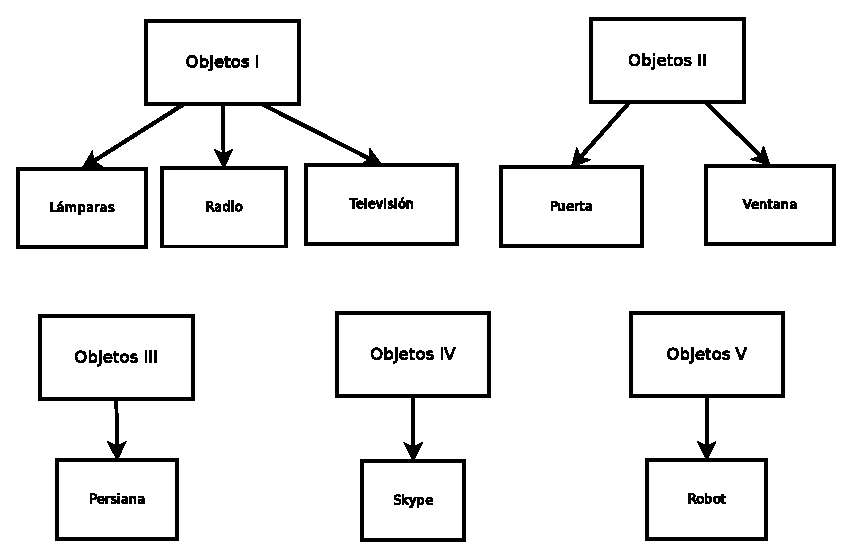
\includegraphics{Esquema_objetos}
  \caption{Clasificación de los objetos para la gramática (aquí también
    se pueden poner acrónimos como \acs{ETTS} y símbolos como \ac{xidet})}
  \label{fig:fig_clobj}
\end{figure}


\subsection{Definición y uso de acrónimos (aquí también
    se pueden poner acrónimos como \acs{ETTS})}
\label{sec:uso-de-acronimos}

El uso del paquete \texttt{glossaries} permite definir los acrónimos y
el sistema automáticamente gestiona su inclusión completa la primera vez
que se usa. Los acrónimos de ejemplo están en el fichero
\texttt{acronyms/defacronymsgl.tex} (con opciones adicionales de
configuración en \texttt{acronyms/acronymsgl.tex}).

Así, si nos referimos a \ac{ETTS} o bien a \ac{EMODB},
veremos como aparecen expandidas la primera vez. A partir de ahí, sólo
se usará el acrónimo como puede verse al volver a hablar de \ac{ETTS} y
\ac{EMODB}.

Tiene también soporte para resetear todos los acrónimos como si no
estuvieran usados. Vuelvo a incluir el párrafo anterior tras un reset
(que se hace con un \texttt{\textbackslash{}glsresetall[acronym]}):

\glsresetall[acronym]

El uso del paquete acronym permite definir los acrónimos y el sistema
automáticamente gestiona su inclusión completa la primera vez que se
usa. Así, si nos referimos a \ac{ETTS} o bien a \ac{EMODB}, veremos como
aparecen expandidas de nuevo (como si fuera la primera vez que se
usan). A partir de ahí, sólo se usará el acrónimo como puede verse al
volver a hablar de \ac{ETTS} y \ac{EMODB}.

Y permite también forzar que se vuelva a citar completo aunque ya se
haya utilizado (con el acrónimo entre paréntesis), como puede verse en
\acl{ETTS} (equivalente a \glsdesc{ETTS} que vale para cualquier
glosario), y también a usar forzosamente el acrónimo. Primero reseteamos
de nuevo.

\glsresetall[acronym]

Y ahora forzamos el acrónimo: \acs{EMODB} (equivalente a
\glsname{EMODB} que vale para cualquier glosario). También podemos
forzar a que lo ponga todo, con \acf{EMODB}.


Podemos seguir definiendo entradas de acrónimos, referirnos a \ac{DBN}
por primera vez, y las siguientes aparecerá como \ac{DBN}.  Pongo ahora
el resto de acrónimos \ac{SQ}, \ac{EIR}, \ac{SIR} y
\ac{ES}. Finalmente los repito para que se vea el efecto: \ac{SQ},
\ac{EIR}, \ac{SIR} y \ac{ES}.

Y gestiona bien los plurales, ponemos el plural como \acp{SOC} la
primera vez, y luego la segunda como \acp{SOC}. Y podemos volver al
singular con \ac{SOC}.


\subsection{Definición y uso de símbolos (aquí también
    se pueden símbolos como \ac{xidet})}
\label{sec:simbolos}

Los símbolos definidos están incluidos en el fichero
\texttt{symbols/defsymbolsgl.tex} (con configuración adicional en
\texttt{symbols/symbolsgl.tex}) y en esta sección mostramos algunos
ejemplos.

El \ac{angstrom} se usa en biología estructural, mientras que el
\ac{ohm} se usa en electrónica. También podemos poner~\ac{xdet}. Y


%%%%%%%%%%%%%%%%%%%%%%%%%%%%%%%%%%%%%%%%%%%%%%%%%%%%%%%%%%%%%%%%%%%%%%%%%%%
%
% Generic template for TFC/TFM/TFG/Tesis
%
% $Id: estudioTeorico.tex,v 1.2 2013/12/12 23:06:55 macias Exp $
%
% By:
%  + Javier Mac�as-Guarasa. 
%    Departamento de Electr�nica
%    Universidad de Alcal�
%  + Roberto Barra-Chicote. 
%    Departamento de Ingenier�a Electr�nica
%    Universidad Polit�cnica de Madrid   
% 
% Based on original sources by Roberto Barra, Manuel Oca�a, Jes�s Nuevo,
% Pedro Revenga, Fernando Herr�nz and Noelia Hern�ndez. Thanks a lot to
% all of them, and to the many anonymous contributors found (thanks to
% google) that provided help in setting all this up.
%
% See also the additionalContributors.txt file to check the name of
% additional contributors to this work.
%
% If you think you can add pieces of relevant/useful examples,
% improvements, please contact us at (macias@depeca.uah.es)
%
% Copyleft 2013
%
%%%%%%%%%%%%%%%%%%%%%%%%%%%%%%%%%%%%%%%%%%%%%%%%%%%%%%%%%%%%%%%%%%%%%%%%%%%

\chapter{Estudio te�rico}
\label{cha:estudio-teorico}

\begin{FraseCelebre}
  \begin{Frase}
    Y as�, del mucho leer y del poco dormir, se le sec� el cerebro de
    manera que vino a perder el juicio\footnote{Tomado de ejemplos del
      proyecto \texis{}.}.
  \end{Frase}
  \begin{Fuente}
    Miguel de Cervantes Saavedra
  \end{Fuente}
\end{FraseCelebre}


\section{Introducci�n}
\label{sec:introduccion-teoria}

En este cap�tulo se cuenta tal y tal.

El cap�tulo se estructura en $n$ apartados\ldots


\section{Estado del Arte}
\label{sec:estadoarte}

En el estado del arte se enumeran los trabajos m�s relevantes de otros
grupos de investigaci�n. A continuaci�n se muestra un ejemplo del uso de
vi�etas que nos proporciona \texttt{itemize}:

\begin{itemize}
\item En el trabajo ..... 
\item En el siguiente trabajo.....
\end{itemize}

O citas en un p�rrafo real: Sin embargo, hay entornos ac�sticos donde
las tasas de error conseguidas son todav�a demasiado altas. En concreto,
las aplicaciones en las que la captura de la se�al de habla se hace
usando micr�fonos alejados del locutor (t�picamente para distancias
superiores a un metro) muestran una fuerte sensibilidad a los problemas
de reverberaci�n, ruido aditivo y baja relaci�n se�al a ruido
(\cite{gelbart02},\cite{kochkin02}). En estos entornos, se ha propuesto
el uso de arrays de micr�fonos como un m�todo para mejorar la calidad
del habla capturada \cite{seltzer03}\cite{herbordt05}.

Existen m�ltiples formas de insertar figuras en Latex. A continuaci�n,
se muestra un ejemplo del uso de \texttt{figure}. Como se puede ver en
la Figura \ref{fig1} tambi�n se pueden poner referencias a las figuras
por medio de \texttt{ref} y la etiqueta \texttt{label} de la figura en
particular.

\begin{figure}[h] %el especificador [h] indica que ponga la figura aqui si es posible
  \centering
  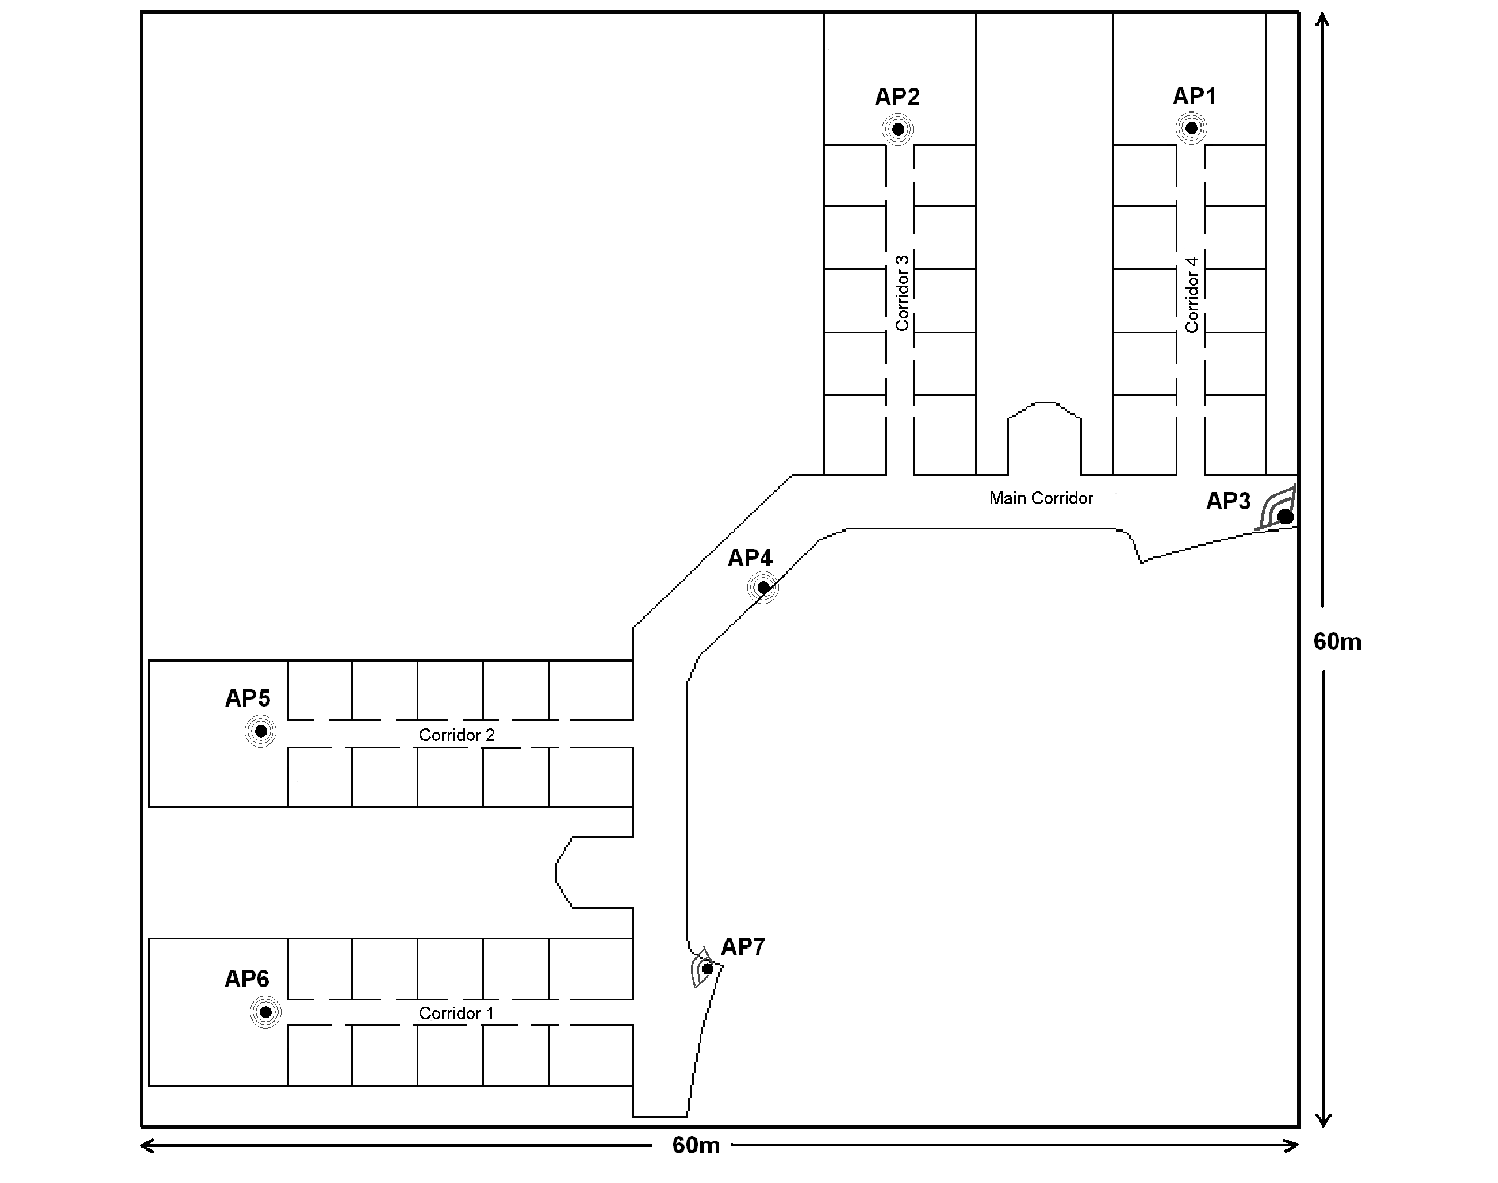
\includegraphics[width=4.7in]{Figure1}
  % where an .eps filename suffix will be assumed under latex, 
  % and a .pdf suffix will be assumed for pdflatex
  \caption{Departamento de Electr�nica.}
  \label{fig1}
\end{figure}

Y ahora un ejemplo en el que ponemos el \texttt{caption} en el lateral:

\begin{SCfigure}
  \centering
  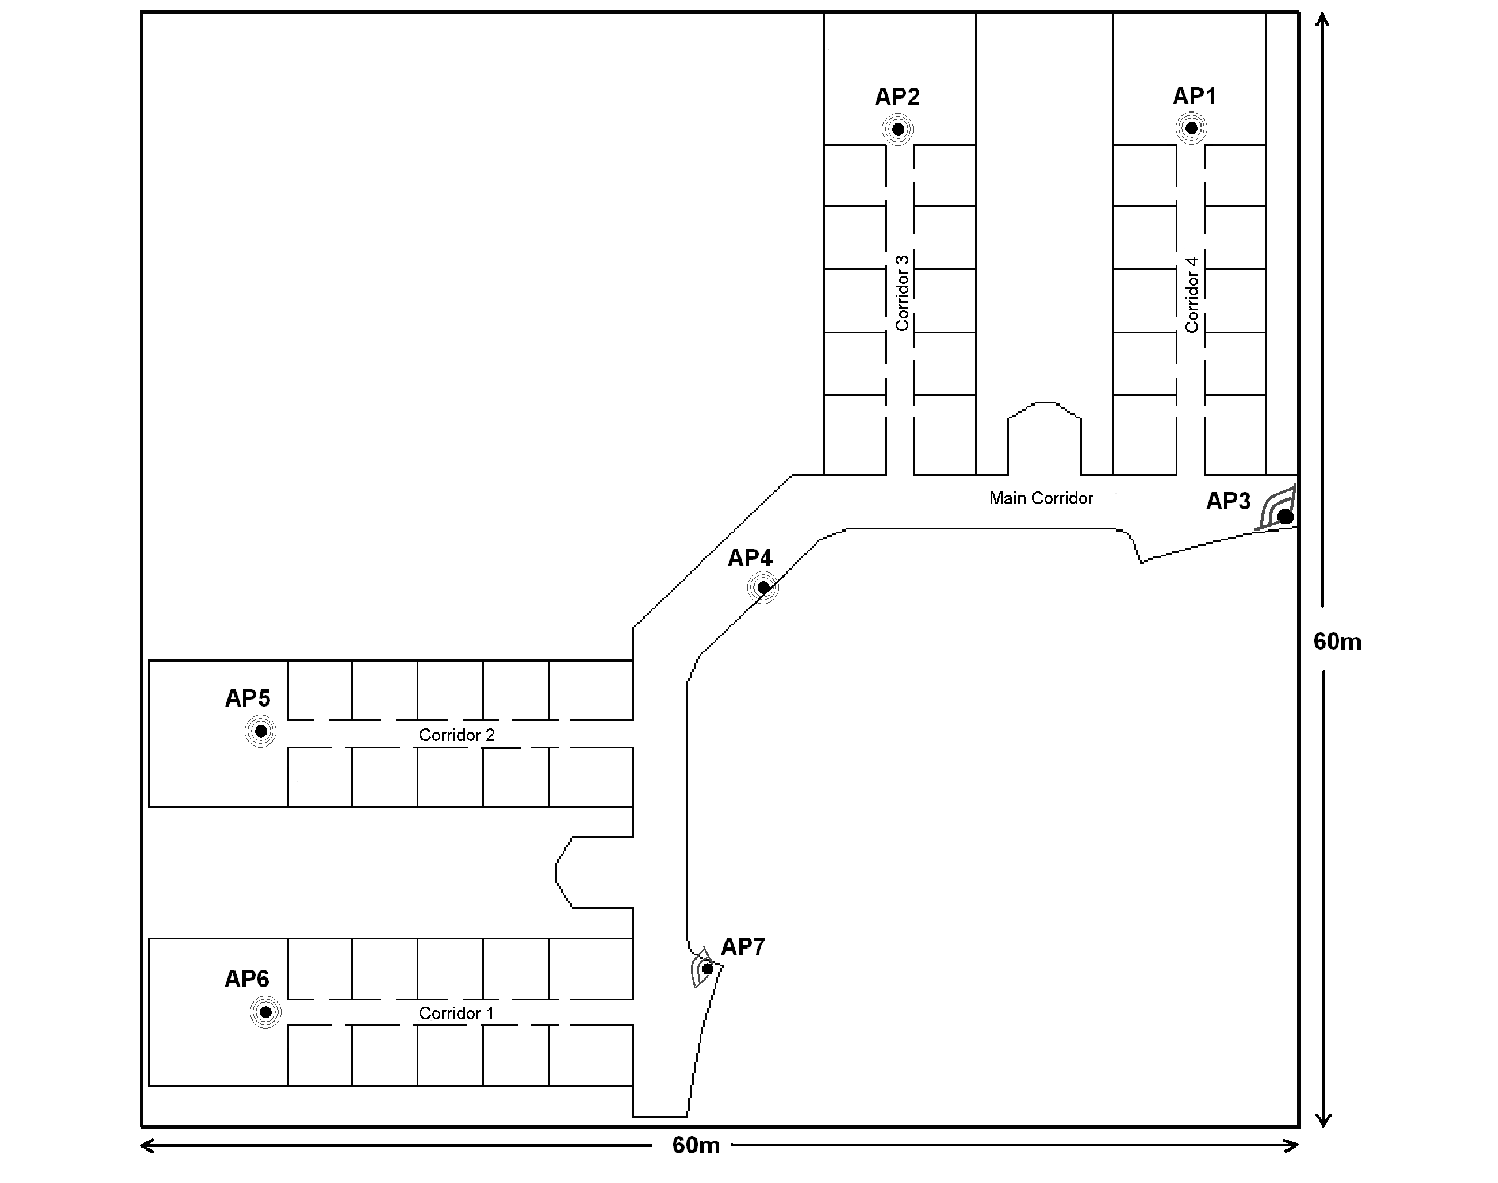
\includegraphics[width=0.5\textwidth]{Figure1}
  \caption{Departamento de Electr�nica en el lateral.}
\end{SCfigure}



\section{T�cnicas utilizadas}
\label{sec:tecnicas-utilizadas}

Blah, blah, blah\ldots


\section{Conclusiones}
\label{sec:conclusiones-teoria}

Blah, blah, blah\ldots

%%% Local Variables:
%%% TeX-master: "../book"
%%% End:


%%%%%%%%%%%%%%%%%%%%%%%%%%%%%%%%%%%%%%%%%%%%%%%%%%%%%%%%%%%%%%%%%%%%%%%%%%%
%
% Generic template for TFC/TFM/TFG/Tesis
%
% $Id: desarrollo.tex,v 1.1 2015/06/05 00:05:19 macias Exp $
%
% By:
%  + Javier Macías-Guarasa. 
%    Departamento de Electrónica
%    Universidad de Alcalá
%  + Roberto Barra-Chicote. 
%    Departamento de Ingeniería Electrónica
%    Universidad Politécnica de Madrid   
% 
% Based on original sources by Roberto Barra, Manuel Ocaña, Jesús Nuevo,
% Pedro Revenga, Fernando Herránz and Noelia Hernández. Thanks a lot to
% all of them, and to the many anonymous contributors found (thanks to
% google) that provided help in setting all this up.
%
% See also the additionalContributors.txt file to check the name of
% additional contributors to this work.
%
% If you think you can add pieces of relevant/useful examples,
% improvements, please contact us at (macias@depeca.uah.es)
%
% You can freely use this template and please contribute with
% comments or suggestions!!!
%
%%%%%%%%%%%%%%%%%%%%%%%%%%%%%%%%%%%%%%%%%%%%%%%%%%%%%%%%%%%%%%%%%%%%%%%%%%%

\chapter{Desarrollo}
\label{cha:development}


\begin{FraseCelebre}
  \begin{Frase}
    A fuerza de construir bien, se llega a buen
    arquitecto\footnote{Tomado de ejemplos del proyecto \texis{}.}.
  \end{Frase}
  \begin{Fuente}
    Aristóteles
  \end{Fuente}
\end{FraseCelebre}



\section{Introducción}
\label{sec:development-introduction}

Blah, blah, blah.

La estructura de este capítulo es\ldots


\section{Sección 1 del capítulo de desarrollo}
\label{sec:development-1}

Blah, blah, blah.


\subsection{Subsección 1.1 del capítulo de desarrollo}
\label{sec:development-11}

Blah, blah, blah.


\subsection{Subsección 1.2 del capítulo de desarrollo}
\label{sec:development-12}

Blah, blah, blah.



\section{Sección 2 del capítulo de desarrollo}
\label{sec:development-2}

Blah, blah, blah.




\section{Conclusiones}
\label{sec:development-conclusions}

Blah, blah, blah.



%%% Local Variables:
%%% TeX-master: "../book"
%%% End:


%%%%%%%%%%%%%%%%%%%%%%%%%%%%%%%%%%%%%%%%%%%%%%%%%%%%%%%%%%%%%%%%%%%%%%%%%%%
%
% Generic template for TFC/TFM/TFG/Tesis
%
% $Id: resultados.tex,v 1.8 2013/11/28 00:15:15 macias Exp $
%
% By:
%  + Javier Mac�as-Guarasa. 
%    Departamento de Electr�nica
%    Universidad de Alcal�
%  + Roberto Barra-Chicote. 
%    Departamento de Ingenier�a Electr�nica
%    Universidad Polit�cnica de Madrid   
% 
% Based on original sources by Roberto Barra, Manuel Oca�a, Jes�s Nuevo,
% Pedro Revenga, Fernando Herr�nz and Noelia Hern�ndez. Thanks a lot to
% all of them, and to the many anonymous contributors found (thanks to
% google) that provided help in setting all this up.
%
% If you think you can add pieces of relevant/useful examples,
% improvements, please contact us at (macias@depeca.uah.es)
%
% Copyleft 2013
%
%%%%%%%%%%%%%%%%%%%%%%%%%%%%%%%%%%%%%%%%%%%%%%%%%%%%%%%%%%%%%%%%%%%%%%%%%%%

\chapter{Resultados}
\label{cha:resultados}


\section{Introducci�n}
\label{sec:introduccion-resultados}

En este cap�tulo se introducir�n los resultados m�s relevantes del
trabajo. 

La estructura del cap�tulo es...


\section{Entorno experimental}
\label{sec:entorno-experimental}

Blah, blah, blah.


\subsection{Bases de datos utilizadas}
\label{sec:bases-de-datos-1}

Blah, blah, blah.


\subsection{M�tricas de calidad}
\label{sec:metricas-de-calidad}

Blah, blah, blah.


\subsection{Estrategia y metodolog�a de experimentaci�n}
\label{sec:estr-y-metod}

Blah, blah, blah.


\section{Resultados experimentales}
\label{sec:result-experim}

A continuaci�n, se muestra un ejemplo de tabla simple (ver tabla \ref{table1}).

\begin{table}
  % increase table row spacing, adjust to taste
  \renewcommand{\arraystretch}{1.3}
  \caption{Comparativa}
  \label{table1}
  \begin{center}
    % Some packages, such as MDW tools, offer better commands for making tables
    % than the plain LaTeX2e tabular which is used here.
    \begin{tabular}{|c|c|c|}
      \hline
      Method & Training Time & Man-Work (\%)\\
      \hline
      Propagation model & $<$ 30 sec & 5\\
      \hline
      Manual & 9 h 30 min & 24\\
      \hline
      Automatic & 2 h & 10 8\\
      \hline
    \end{tabular}
  \end{center}
\end{table}

Cuando las tablas ocupan m�s de un p�gina se debe utilizar un tipo
especial de tablas denominado ''longtbale''. A continuaci�n, se muestra
un ejemplo del mismo (ver tabla \ref{table2}).

\begin{center}
	\begin{longtable}{|c|c|c|c|}
    \caption[Resultados de la Correlacion cruzada]{Resultados de la Correlaci�n cruzada} \label{table2} \\
    
    \hline \multicolumn{1}{|c|}{\textbf{Posici�n Real}} & \multicolumn{1}{c|}{\textbf{Posici�n estimada}} & \multicolumn{1}{c|}{\textbf{Coef. Correlaci�n}} & \multicolumn{1}{c|}{\textbf{Acierto/Fallo}} \\ \hline 
    \endfirsthead
    
    \multicolumn{4}{c}%
    {{\bfseries \tablename\ \thetable{} -- continua en la p�gina anterior}} \\
    \hline \multicolumn{1}{|c|}{\textbf{Posici�n Real}} & \multicolumn{1}{c|}{\textbf{Posici�n estimada}} & \multicolumn{1}{c|}{\textbf{Coef. Correlaci�n}} & \multicolumn{1}{c|}{\textbf{Acierto/Fallo}} \\ \hline 
    \endhead
    
    \hline \multicolumn{4}{|r|}{{Continua en la p�gina siguiente}} \\ \hline
    \endfoot
    \hline \hline
    \endlastfoot
    
    \hline	2P0	&	2P0	&	0,004954	&	A	\\
    \hline	2P1	&	2P4	&	0,005752	&	F	\\
    \hline	2P2	&	2P2	&	0,005461	&	A	\\
    \hline	2P3	&	2P0	&	0,004634	&	F	\\
    \hline	2P5	&	2P4	&	0,005991	&	F	\\
    \hline	2P6	&	2P16	&	0,004410	&	F	\\
    \hline	2P7	&	3P9	&	0,008038	&	F	\\
    \hline	2P8	&	3P9	&	0,003753	&	F	\\
    \hline	2P9	&	2P7	&	0,004908	&	F	\\
    \hline	2P10	&	2P10	&	0,007273	&	A	\\
    \hline	2P14	&	2P16	&	0,006485	&	F	\\
    \hline	2P15	&	2P15	&	0,004932	&	A	\\
    \hline	2P16	&	2P16	&	0,006237	&	A	\\
    \hline	2P17	&	2P15	&	0,005110	&	F	\\
    \hline	2P18	&	3P18	&	0,006235	&	F	\\
    \hline	2P19	&	3P18	&	0,004827	&	F	\\
    \hline	2P20	&	2P20	&	0,006877	&	A	\\
    \hline	2P22	&	3P18	&	0,003048	&	F	\\
    \hline	2P24	&	2P24	&	0,006833	&	A	\\
    \hline	2P25	&	2P25	&	0,004875	&	A	\\
    \hline	2P26	&	2P31	&	0,005511	&	F	\\
    \hline	2P27	&	2P28	&	0,004590	&	F	\\
    \hline	2P30	&	2P31	&	0,005576	&	F	\\
    \hline	2P31	&	2P31	&	0,007213	&	A	\\
    \hline	2P32	&	2P35	&	0,003340	&	F	\\
    \hline	2P34	&	2P34	&	0,004128	&	A	\\
    \hline	2P36	&	2P35	&	0,003329	&	F	\\
    \hline	2P37	&	2P37	&	0,003468	&	A	\\
    \hline	2P39	&	2P38	&	0,002577	&	F	\\
    \hline	2P40	&	2P43	&	0,004303	&	F	\\
    \hline	2P41	&	2P41	&	0,001573	&	A	\\
    \hline	2P42	&	2P41	&	0,000846	&	F	\\
    \hline	2P44	&	2P44	&	0,002732	&	A	\\
    \hline	2P45	&	23P45	&	0,001958	&	F	\\
    \hline	2P47	&	2P34	&	0,002869	&	F	\\
    \hline	2P48	&	2P43	&	0,004569	&	F	\\
    \hline	2P49	&	3P51	&	0,001374	&	F	\\
    \hline	2P50	&	2P34	&	0,002274	&	F	\\
    \hline	2P51	&	2P63	&	0,003931	&	F	\\
    \hline	2P52	&	2P55	&	0,003537	&	F	\\
    \hline	2P53	&	3P56	&	0,003126	&	F	\\
    \hline	2P54	&	2P67	&	0,005560	&	F	\\
    \hline	2P56	&	2P55	&	0,002817	&	F	\\
    \hline	2P57	&	2P67	&	0,006168	&	F	\\
    \hline	2P58	&	2P58	&	0,005278	&	A	\\
    \hline	2P60	&	3P66	&	0,004966	&	F	\\
    \hline	2P61	&	3P61	&	0,004748	&	A	\\
    \hline	2P64	&	2P67	&	0,005342	&	F	\\
    \hline	2P66	&	2P4	&	0,004172	&	F	\\
    \hline	2P67	&	2P67	&	0,005706	&	A	\\
    \hline	3P0	&	3P0	&	0,003674	&	A	\\
    \hline	3P61	&	2P61	&	0,003263	&	F	\\
    \hline	3P64	&	2P67	&	0,003484	&	F	\\
    \hline	3P65	&	2P67	&	0,002975	&	F	\\
    \hline	3P66	&	2P58	&	0,005029	&	F	\\
    \hline	3P67	&	3P67	&	0,003714	&	A	\\
	\end{longtable}
\end{center}

En algunas ocasiones, tambi�n resulta �til emplear el entorno
''subfloat'' (del nuevo paquete subfig) para a�adir m�ltiples im�genes
dentro de la misma figura. A continuaci�n, se muestra un ejemplo del uso
en la figura \ref{fig:fig2}. Tambi�n se pueden referenciar las
sub-figuras de forma individual, por ejemplo la sub-figura
\ref{fig:fig2b} (usando un m�todo de cita), o bien la sub-figura
\ref{fig:fig2}\subref{fig:fig2b} (usando otro).

\begin{figure}[h]
  \centerline{\subfloat[Mean entropy]{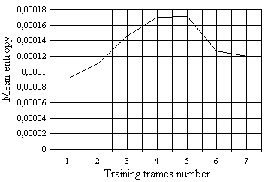
\includegraphics[width=3in]{Figure2}
      % where an .eps filename suffix will be assumed under latex, 
      % and a .pdf suffix will be assumed for pdflatex
      \label{fig:fig2a}}
    \hfil
    \subfloat[Error Percentage]{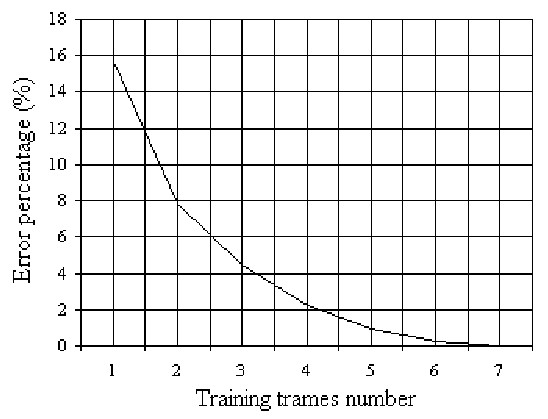
\includegraphics[width=2.7in]{Figure3}
      % where an .eps filename suffix will be assumed under latex, 
      % and a .pdf suffix will be assumed for pdflatex
      \label{fig:fig2b}}}
  \caption{Optimal trames number in the training data set}
  \label{fig:fig2}
\end{figure}

% For this to work you need to (in preamble.tex):
% - remove \usepackage{subfig}
% - add \usepackage{caption}
% - add \usepackage{subcaption}
% \begin{figure}
%   \centering
%   \begin{subfigure}[b]{0.3\textwidth}
%     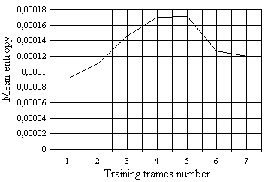
\includegraphics[width=\textwidth]{Figure2}
%     \caption{Mean Entropy}
%     \label{fig:fig3a}
%   \end{subfigure}%
%   ~ %add desired spacing between images, e. g. ~, \quad, \qquad etc.
%   % (or a blank line to force the subfigure onto a new line)
%   \begin{subfigure}[b]{0.3\textwidth}
%     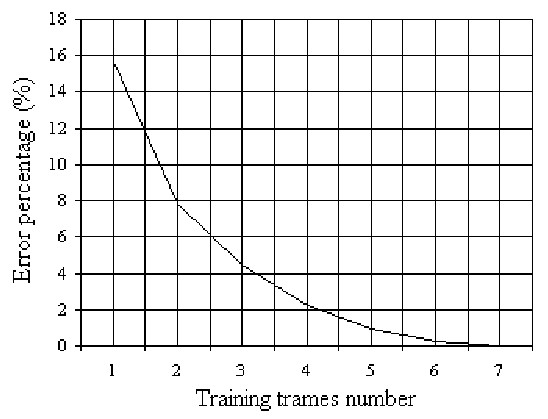
\includegraphics[width=\textwidth]{Figure3}
%     \caption{Error Percentage}
%     \label{fig:fig3b}
%   \end{subfigure}
%   \caption{Optimal trames number in the training data set}
%   \label{fig:fig3}
% \end{figure}

Incluso podemos poner una tabla ``apaisada'', como en la
\ref{tablas2006}, donde se muestra un resumen de los resultados
obtenidos en una serie de experimentos de localizaci�n de locutores.

\clearpage
% \begin{table}[H]\centering
\begin{sidewaystable}[hbtp]
  \begin{center}

    \begin{tabular}{||l|c|c|c|c|c||}
      \hline \hline
      & UKA & ITC & AIT & UPC & IBM\\
      \hline
      \hline
      Pcor & $57.0\pm1.4\%$ & $84.0\pm3.3\%$ & $47.0\pm3.1\%$ & $20.0\pm2.5\%$ & $67.0\pm2.9\%$ \\
      \hline
      Bias fine (x:y:z) [mm] & $20:-42:-75$ & $45:27:-41$ & $-27:-77:-40$ & $-59:112:52$ & $91:-69:-38$ \\
      \hline
      Bias fine+gross (x,y,z) [mm] & $735:-93:-258$ & $67:439:-134$ & $17:-402:-118$ & $-141:255:39$ & $474:-141:-14$ \\
      \hline
      AEE fine [mm] = MOTP & $210$ & $130$ & $266$ & $344$ & $228$ \\
      \hline
      Fine+gross [mm] & $1201$ & $632$ & $1006$ & $1188$ & $884$ \\
      \hline
      Loc. frames & $5035$ & $22$ & $995$ & $977$ & $1023$ \\
      \hline
      Ref. duration (s) & $6287.0$ & $596.0$ & $1143.0$ & $1180.0$ & $1194.0$ \\
      \hline \hline
    \end{tabular}
    \caption{Resultados TEST CLEAR 2006}
    \label{tablas2006}
  \end{center}
\end{sidewaystable}
% \end{table}


\section{Conclusiones}
\label{sec:conclusiones-resultados}

Blah, blah, blah.

%%% Local Variables:
%%% TeX-master: "../book"
%%% End:


%%%%%%%%%%%%%%%%%%%%%%%%%%%%%%%%%%%%%%%%%%%%%%%%%%%%%%%%%%%%%%%%%%%%%%%%%%%
%
% Generic template for TFC/TFM/TFG/Tesis
%
% $Id: conclusiones.tex,v 1.1 2015/06/05 00:05:20 macias Exp $
%
% By:
%  + Javier Macías-Guarasa. 
%    Departamento de Electrónica
%    Universidad de Alcalá
%  + Roberto Barra-Chicote. 
%    Departamento de Ingeniería Electrónica
%    Universidad Politécnica de Madrid   
% 
% Based on original sources by Roberto Barra, Manuel Ocaña, Jesús Nuevo,
% Pedro Revenga, Fernando Herránz and Noelia Hernández. Thanks a lot to
% all of them, and to the many anonymous contributors found (thanks to
% google) that provided help in setting all this up.
%
% See also the additionalContributors.txt file to check the name of
% additional contributors to this work.
%
% If you think you can add pieces of relevant/useful examples,
% improvements, please contact us at (macias@depeca.uah.es)
%
% You can freely use this template and please contribute with
% comments or suggestions!!!
%
%%%%%%%%%%%%%%%%%%%%%%%%%%%%%%%%%%%%%%%%%%%%%%%%%%%%%%%%%%%%%%%%%%%%%%%%%%%

\chapter{Conclusiones y líneas futuras}
\label{cha:concl-y-line}

En este apartado se resumen las conclusiones obtenidas y se proponen
futuras líneas de investigación que se deriven del trabajo.

La estructura del capítulo es...


\section{Conclusiones}
\label{sec:conclusiones}

Para añadir una referencia a un autor, se puede utilizar el paquete
\texttt{cite}. En el trabajo \cite{armani03}, se muestra un trabajo...

Y podemos usar de nuevo algún acrónimo, como por ejemplo \ac{TDPSOLA}, o
uno ya referenciado como \ac{ANN}.


\section{Líneas futuras}
\label{sec:lineas-futuras}

Pues eso.


%%% Local Variables:
%%% TeX-master: "../book"
%%% End:




% Optional in PFCs
%%%%%%%%%%%%%%%%%%%%%%%%%%%%%%%%%%%%%%%%%%%%%%%%%%%%%%%%%%%%%%%%%%%%%%%%%%%%
%
% Generic template for TFC/TFM/TFG/Tesis
%
% $Id: pliego.tex,v 1.2 2013/11/04 23:46:21 macias Exp $
%
% By:
%  + Javier Mac�as-Guarasa. 
%    Departamento de Electr�nica
%    Universidad de Alcal�
%  + Roberto Barra-Chicote. 
%    Departamento de Ingenier�a Electr�nica
%    Universidad Polit�cnica de Madrid   
% 
% Based on original sources by Roberto Barra, Manuel Oca�a, Jes�s Nuevo,
% Pedro Revenga, Fernando Herr�nz and Noelia Hern�ndez. Thanks a lot to
% all of them, and to the many anonymous contributors found (thanks to
% google) that provided help in setting all this up.
%
% If you think you can add pieces of relevant/useful examples,
% improvements, please contact us at (macias@depeca.uah.es)
%
% Copyleft 2013
%
%%%%%%%%%%%%%%%%%%%%%%%%%%%%%%%%%%%%%%%%%%%%%%%%%%%%%%%%%%%%%%%%%%%%%%%%%%%

\chapter{Pliego de condiciones}
\label{cha:pliego-de-condiciones}

Blah, blah, blah.

%%% Local Variables:
%%% TeX-master: "../book"
%%% End:


% Optional in PFCs, compulsory in TFGs
%%%%%%%%%%%%%%%%%%%%%%%%%%%%%%%%%%%%%%%%%%%%%%%%%%%%%%%%%%%%%%%%%%%%%%%%%%%%
%
% Generic template for TFC/TFM/TFG/Tesis
%
% $Id: presupuesto.tex,v 1.3 2013/11/25 00:33:32 macias Exp $
%
% By:
%  + Javier Mac�as-Guarasa. 
%    Departamento de Electr�nica
%    Universidad de Alcal�
%  + Roberto Barra-Chicote. 
%    Departamento de Ingenier�a Electr�nica
%    Universidad Polit�cnica de Madrid   
% 
% Based on original sources by Roberto Barra, Manuel Oca�a, Jes�s Nuevo,
% Pedro Revenga, Fernando Herr�nz and Noelia Hern�ndez. Thanks a lot to
% all of them, and to the many anonymous contributors found (thanks to
% google) that provided help in setting all this up.
%
% See also the additionalContributors.txt file to check the name of
% additional contributors to this work.
%
% If you think you can add pieces of relevant/useful examples,
% improvements, please contact us at (macias@depeca.uah.es)
%
% Copyleft 2013
%
%%%%%%%%%%%%%%%%%%%%%%%%%%%%%%%%%%%%%%%%%%%%%%%%%%%%%%%%%%%%%%%%%%%%%%%%%%%

\chapter{Presupuesto}
\label{cha:presupuesto}

Blah, blah, blah.

%%% Local Variables:
%%% TeX-master: "../book"
%%% End:


%%%%%%%%%%%%%%%%%%%%%%%%%%%%%%%%%%%%%%%%%%%%%%%%%%%%%%%%%%%%%%%%%%%%%%%%%%%
% Bibliography
%%%%%%%%%%%%%%%%%%%%%%%%%%%%%%%%%%%%%%%%%%%%%%%%%%%%%%%%%%%%%%%%%%%%%%%%%%%
%%%%%%%%%%%%%%%%%%%%%%%%%%%%%%%%%%%%%%%%%%%%%%%%%%%%%%%%%%%%%%%%%%%%%%%%%%%
%
% Generic template for TFC/TFM/TFG/Tesis
%
% $Id: bibliography.tex,v 1.7 2014/01/08 22:56:04 macias Exp $
%
% By:
%  + Javier Mac�as-Guarasa. 
%    Departamento de Electr�nica
%    Universidad de Alcal�
%  + Roberto Barra-Chicote. 
%    Departamento de Ingenier�a Electr�nica
%    Universidad Polit�cnica de Madrid   
% 
% Based on original sources by Roberto Barra, Manuel Oca�a, Jes�s Nuevo,
% Pedro Revenga, Fernando Herr�nz and Noelia Hern�ndez. Thanks a lot to
% all of them, and to the many anonymous contributors found (thanks to
% google) that provided help in setting all this up.
%
% See also the additionalContributors.txt file to check the name of
% additional contributors to this work.
%
% If you think you can add pieces of relevant/useful examples,
% improvements, please contact us at (macias@depeca.uah.es)
%
% Copyleft 2013
%
%%%%%%%%%%%%%%%%%%%%%%%%%%%%%%%%%%%%%%%%%%%%%%%%%%%%%%%%%%%%%%%%%%%%%%%%%%%

%\bibliographystyle{plainnat}
%\bibliographystyle{dinat}
%\bibliographystyle{unsrt}
\bibliographystyle{IEEEtran}

% The following is overly complicated because I was not able to do so in
% another way. The problem is the bibliography command being "called"
% from both the root and anteproyecto directories...
%
% Here define as many bibfiles as needed
\newcommand{\mybibfileOne}{biblio/biblio}
\newcommand{\mybibfileTwo}{biblio/biblio2}
%...
%\newcommand{\mybibfileN}{biblio/biblioN}

% This is for a single bib file
\newcommand{\mybibfiles}{\myreferencespath\mybibfileOne}
% but do this for multiple files
%\newcommand{\mybibfiles}{\myreferencespath\mybibfile1,\myreferencespath\mybibfile2,...,\myreferencespath\mybibfileN}

% Do not touch this
\bibliography{\mybibfiles}


%%% Local Variables:
%%% TeX-master: "../book"
%%% End:





%%%%%%%%%%%%%%%%%%%%%%%%%%%%%%%%%%%%%%%%%%%%%%%%%%%%%%%%%%%%%%%%%%%%%%%%%%%
% Appendices
%%%%%%%%%%%%%%%%%%%%%%%%%%%%%%%%%%%%%%%%%%%%%%%%%%%%%%%%%%%%%%%%%%%%%%%%%%%
% I don't recommend it, but if you want to define "parts", use this...
% BEWARE: I didn't write the english dependent code
%\part*{Ap�ndices}
%\label{part:apendices}

\appendix

%%%%%%%%%%%%%%%%%%%%%%%%%%%%%%%%%%%%%%%%%%%%%%%%%%%%%%%%%%%%%%%%%%%%%%%%%%%
%
% Generic template for TFC/TFM/TFG/Tesis
%
% $Id:$
%
% By:
%  + Javier Mac�as-Guarasa. 
%    Departamento de Electr�nica
%    Universidad de Alcal�
%  + Roberto Barra-Chicote. 
%    Departamento de Ingenier�a Electr�nica
%    Universidad Polit�cnica de Madrid   
% 
% Based on original sources by Roberto Barra, Manuel Oca�a, Jes�s Nuevo,
% Pedro Revenga, Fernando Herr�nz and Noelia Hern�ndez. Thanks a lot to
% all of them, and to the many anonymous contributors found (thanks to
% google) that provided help in setting all this up.
%
% If you think you can add pieces of relevant/useful examples,
% improvements, please contact us at (macias@depeca.uah.es)
%
% (copyleft)2013
%
%%%%%%%%%%%%%%%%%%%%%%%%%%%%%%%%%%%%%%%%%%%%%%%%%%%%%%%%%%%%%%%%%%%%%%%%%%%

\chapter{Manual de usuario}
\label{cha:concl-y-line}

\section{Introducci�n}
\label{sec:introapp1}


Introducci�n.

\section{Manual}
\label{sec:manual}

Pues eso.


%%%%%%%%%%%%%%%%%%%%%%%%%%%%%%%%%%%%%%%%%%%%%%%%%%%%%%%%%%%%%%%%%%%%%%%%%%%
%
% Generic template for TFC/TFM/TFG/Tesis
%
% $Id: herramientas.tex,v 1.3 2013/11/04 23:46:21 macias Exp $
%
% By:
%  + Javier Mac�as-Guarasa. 
%    Departamento de Electr�nica
%    Universidad de Alcal�
%  + Roberto Barra-Chicote. 
%    Departamento de Ingenier�a Electr�nica
%    Universidad Polit�cnica de Madrid   
% 
% Based on original sources by Roberto Barra, Manuel Oca�a, Jes�s Nuevo,
% Pedro Revenga, Fernando Herr�nz and Noelia Hern�ndez. Thanks a lot to
% all of them, and to the many anonymous contributors found (thanks to
% google) that provided help in setting all this up.
%
% If you think you can add pieces of relevant/useful examples,
% improvements, please contact us at (macias@depeca.uah.es)
%
% Copyleft 2013
%
%%%%%%%%%%%%%%%%%%%%%%%%%%%%%%%%%%%%%%%%%%%%%%%%%%%%%%%%%%%%%%%%%%%%%%%%%%%

\chapter{Herramientas y recursos}
\label{cha:herr-y-recurs}

Las herramientas necesarias para la elaboraci�n del proyecto han sido:

\begin{itemize}
\item PC compatible 
\item Sistema operativo GNU/Linux \cite{gnulinux}
\item Entorno de desarrollo Emacs \cite{emacs}
\item Entorno de desarrollo KDevelop \cite{kdevelop}
\item Procesador de textos \LaTeX \cite{lamport94}
\item Lenguaje de procesamiento matem�tico Octave  \cite{octave}
\item Control de versiones CVS \cite{cvs}
\item Compilador C/C++ gcc \cite{gcc}
\item Gestor de compilaciones make \cite{make}
\end{itemize}

%%% Local Variables:
%%% TeX-master: "../book"
%%% End:




\backmatter

% Just for TFGs at UAH right now, but kept here
%%%%%%%%%%%%%%%%%%%%%%%%%%%%%%%%%%%%%%%%%%%%%%%%%%%%%%%%%%%%%%%%%%%%%%%%%%%
%
% Generic template for TFC/TFM/TFG/Tesis
%
% $Id: backpage.tex,v 1.6 2018/12/12 15:29:21 macias Exp $
%
% By:
%  + Javier Macías-Guarasa. 
%    Departamento de Electrónica
%    Universidad de Alcalá
%  + Roberto Barra-Chicote. 
%    Departamento de Ingeniería Electrónica
%    Universidad Politécnica de Madrid   
% 
% Based on original sources by Roberto Barra, Manuel Ocaña, Jesús Nuevo,
% Pedro Revenga, Fernando Herránz and Noelia Hernández. Thanks a lot to
% all of them, and to the many anonymous contributors found (thanks to
% google) that provided help in setting all this up.
%
% See also the additionalContributors.txt file to check the name of
% additional contributors to this work.
%
% If you think you can add pieces of relevant/useful examples,
% improvements, please contact us at (macias@depeca.uah.es)
%
% You can freely use this template and please contribute with
% comments or suggestions!!!
%
%%%%%%%%%%%%%%%%%%%%%%%%%%%%%%%%%%%%%%%%%%%%%%%%%%%%%%%%%%%%%%%%%%%%%%%%%%%

%%%%%%%%%%%%%%%%%%%%%%%%%%%%%%%%%%%%%%%%%%%%%%%%%%%%%%%%%%%%%%%%%%%%%%%%%%%
% Right now (november 2013), it's only defined for TFGs at UAH
%%%%%%%%%%%%%%%%%%%%%%%%%%%%%%%%%%%%%%%%%%%%%%%%%%%%%%%%%%%%%%%%%%%%%%%%%%%

\ifthenelse{\equal{\mybookworktype}{TFG}}
{
  %%%%%%%%%%%%%%%%%%%%%%%%%%%%%%%%%%%%%%%%%%%%%%%%%%%%%%%%%%%%%%%%%%%%%%%%%%%
%
% Generic template for TFC/TFM/TFG/Tesis
%
% $Id: backpage-tfg-uah.tex,v 1.5 2013/11/25 00:33:31 macias Exp $
%
% By:
%  + Javier Mac�as-Guarasa. 
%    Departamento de Electr�nica
%    Universidad de Alcal�
%  + Roberto Barra-Chicote. 
%    Departamento de Ingenier�a Electr�nica
%    Universidad Polit�cnica de Madrid   
% 
% Based on original sources by Roberto Barra, Manuel Oca�a, Jes�s Nuevo,
% Pedro Revenga, Fernando Herr�nz and Noelia Hern�ndez. Thanks a lot to
% all of them, and to the many anonymous contributors found (thanks to
% google) that provided help in setting all this up.
%
% See also the additionalContributors.txt file to check the name of
% additional contributors to this work.
%
% If you think you can add pieces of relevant/useful examples,
% improvements, please contact us at (macias@depeca.uah.es)
%
% Copyleft 2013
%
%%%%%%%%%%%%%%%%%%%%%%%%%%%%%%%%%%%%%%%%%%%%%%%%%%%%%%%%%%%%%%%%%%%%%%%%%%%

% This is a trick to avoid the header to be shown. There must be a
% better way...
\chapter*{ }
\thispagestyle{empty}

\cleartoleftpage
\thispagestyle{empty}

% To add background watermark, defined in config/preamble.tex
\BgThispage

% Nice example of tikz
% \begin{tikzpicture}[remember picture,overlay]
%   \node [xshift=1cm,yshift=1cm] at (current page.south west)
%   [text width=7cm,fill=red!20,rounded corners,above right]
%   {
%     This is an absolutely positioned text in the
%     lower left corner. No shipout-hackery is used.
%   };
% \end{tikzpicture}

\begin{tikzpicture}[remember picture,overlay]
    \node[yshift=-5cm] at (current page.north west)
      {
        \begin{tikzpicture}[remember picture, overlay]
          \draw[fill=headingPortadaTFM] (0,0) rectangle (\paperwidth,5cm);
          \node [yshift=3cm, xshift=0.5\paperwidth, font=\Huge, text centered, midway] {\color{textoHeadingPortadaTFM}Universidad de Alcal�};
          \node [yshift=2cm, xshift=0.5\paperwidth, font=\Huge, text centered, midway] {\color{textoHeadingPortadaTFM}Escuela Polit�cnica Superior};

        \end{tikzpicture}
      };
   \end{tikzpicture}


\large
\vspace{20cm}
\begin{center}
  
  \centerline{
\includegraphics[height=2.5cm]{logoUAH.jpg}}

\end{center}



%%% Local Variables:
%%% TeX-master: "../book"
%%% End:



}
{
\ifthenelse{\equal{\mybookworktype}{TFM}}
{
  %%%%%%%%%%%%%%%%%%%%%%%%%%%%%%%%%%%%%%%%%%%%%%%%%%%%%%%%%%%%%%%%%%%%%%%%%%%
%
% Generic template for TFC/TFM/TFG/Tesis
%
% $Id: backpage-tfg-uah.tex,v 1.5 2013/11/25 00:33:31 macias Exp $
%
% By:
%  + Javier Mac�as-Guarasa. 
%    Departamento de Electr�nica
%    Universidad de Alcal�
%  + Roberto Barra-Chicote. 
%    Departamento de Ingenier�a Electr�nica
%    Universidad Polit�cnica de Madrid   
% 
% Based on original sources by Roberto Barra, Manuel Oca�a, Jes�s Nuevo,
% Pedro Revenga, Fernando Herr�nz and Noelia Hern�ndez. Thanks a lot to
% all of them, and to the many anonymous contributors found (thanks to
% google) that provided help in setting all this up.
%
% See also the additionalContributors.txt file to check the name of
% additional contributors to this work.
%
% If you think you can add pieces of relevant/useful examples,
% improvements, please contact us at (macias@depeca.uah.es)
%
% Copyleft 2013
%
%%%%%%%%%%%%%%%%%%%%%%%%%%%%%%%%%%%%%%%%%%%%%%%%%%%%%%%%%%%%%%%%%%%%%%%%%%%

% This is a trick to avoid the header to be shown. There must be a
% better way...
\chapter*{ }
\thispagestyle{empty}

\cleartoleftpage
\thispagestyle{empty}

% To add background watermark, defined in config/preamble.tex
\BgThispage

% Nice example of tikz
% \begin{tikzpicture}[remember picture,overlay]
%   \node [xshift=1cm,yshift=1cm] at (current page.south west)
%   [text width=7cm,fill=red!20,rounded corners,above right]
%   {
%     This is an absolutely positioned text in the
%     lower left corner. No shipout-hackery is used.
%   };
% \end{tikzpicture}

\begin{tikzpicture}[remember picture,overlay]
    \node[yshift=-5cm] at (current page.north west)
      {
        \begin{tikzpicture}[remember picture, overlay]
          \draw[fill=headingPortadaTFM] (0,0) rectangle (\paperwidth,5cm);
          \node [yshift=3cm, xshift=0.5\paperwidth, font=\Huge, text centered, midway] {\color{textoHeadingPortadaTFM}Universidad de Alcal�};
          \node [yshift=2cm, xshift=0.5\paperwidth, font=\Huge, text centered, midway] {\color{textoHeadingPortadaTFM}Escuela Polit�cnica Superior};

        \end{tikzpicture}
      };
   \end{tikzpicture}


\large
\vspace{20cm}
\begin{center}
  
  \centerline{
\includegraphics[height=2.5cm]{logoUAH.jpg}}

\end{center}



%%% Local Variables:
%%% TeX-master: "../book"
%%% End:



}
{
}
}

%%% Local Variables:
%%% TeX-master: "../book"
%%% End:




\end{document}

